%\documentclass{beamer}
%\usepackage{amsmath}
%\usepackage{amsfonts}
%\usepackage{amsthm}
%\usepackage{amssymb}
%\usepackage{tikz}
%\usetikzlibrary{trees}
%\usepackage{lipsum}

%===== main document class =====
%\ifdefined\slideModeHandout
\documentclass%
[%
  handout,          % avoid unnecessary overlays
  aspectratio=169,  % aspect ratio fo 16:9 
  t,                % place content at top of frames
  10pt,             % use 10pt as standard font size (default size is 11pt)
  compress,         % compress things like navigation bars...
]{beamer}
%\else
%\documentclass%
%[%
%  aspectratio=169,  % aspect ratio fo 16:9 
%  t,                % place content at top of frames
%  10pt,             % use 10pt as standard font size (default size is 11pt)
%  compress,         % compress things like navigation bars...
%]{beamer}
%\fi

\mode<presentation>
%===============tabto==============
% tabto.sty
%
% version 1.4  (Dec 2018)
%
% Tabbing to fixed positions in a paragraph.
%
% Copyright 2006,2009,2012,2013,2018 by 
% Donald Arseneau,   Vancouver, Canada (asnd@triumf.ca)
% Permission to use, distribute and modify this software is granted
% under the conditions of the LaTeX Project Public License, either 
% version 1.3 or (at your option) any later version.  The license is
% found at http://www.latex-project.org/lppl.txt, and is part of all 
% recent distributions of LaTeX.
%
% This work has the LPPL maintenance status `maintained' (by author).
%
% Two new text positioning commands are defined: \tabto and \tab.
% 
% \tabto{<length>}
% Tab to a position relative to the left margin in a paragraph (any
% indentation due to a list or \leftskip is part of the `margin' in
% this context). If the text on the line already goes past the desired
% position, the tab starts a new line and moves to the requested
% horizontal position.
%
% \tabto*{<length>}
% Similar to \tabto, except it will perform backspacing, and over-
% print previous text on the line whenever that text is already
% longer than the specified length (i.e., no linebreak is produced).
% Line-breaks are suppressed immediately after \tabto or \tabto*.
%
% The length register "\CurrentLineWidth" will report the width
% of the existing text on the line, and it may be used in the
% <length> argument (using calc.sty, for example). Also, there
% is "\TabPrevPos" which gives the "\CurrentLineWidth" from the
% previous tab command (the position where the tab command occurred,
% not where it went to), and can be used to return to that position
% if no line breaks have occurred in between, or directly below it,
% if there were line breaks.
%
% \tab
% Tab to the next tab-stop chosen from a list of tab positions, in
% the traditional style of typewriters.  A \tab will always move
% to the next tab stop (or the next line), even if it is already
% exactly at a tab stop. Thus, "\tab" at the beginning of a line,
% or "\tab\tab" elsewhere skips a position. A linebreak is permitted 
% immediately following a \tab, in case the ensuing text does not 
% fit well in the remaining space.
%
% If you do not want to skip positions, use "\tabto{\NextTabStop}"
% instead of "\tab".  This is particularly useful when you want to
% use \tab in some other command, but do not want to skip a column
% for the first item.
%
% The tab-stop positions are declared using either \TabPositions
% or \NumTabs:
%
% \TabPositions{<length>, <length>,...<length>}
% Declares the tab stops as a comma-separated list of positions 
% relative to the left margin. A tab-stop at 0pt is implicit, and 
% need not be listed.
%
% \NumTabs{<number>}
% Declares a list of <number> equally-spaced tabs, starting at the
% left margin and spanning \linewidth.  For example \NumTabs{2} 
% declares tab-stops at 0pt and 0.5\linewidth, the same as
% \TabPositions{0pt, 0.5\linewidth} or \TabPositions{0.5\linewidth}
%
% After these declarations, the list of tab positions is saved in
% \TabStopList, and the next tab position, relative to the current 
% position, is given by \NextTabStop.  You do not normally need
% to access them, but they are available.
%
% Problems:
%
% Tall objects after a tab stop may overlap the line above, rather
% than forcing a greater separation between lines.

%\ProvidesPackage{tabto}[2018/12/28 \space v 1.4 \space 
%  Another tabbing mechanism]\relax

%%%%%%%%%Code Begin

%\newdimen\CurrentLineWidth
%\newdimen\TabPrevPos
%
%\newcommand\tabto[1]{%
% \leavevmode
% \begingroup
% \def\@tempa{*}\def\@tempb{#1}%
% \ifx\@tempa\@tempb % \tab* 
%   \endgroup
%   \TTo@overlaptrue % ... set a flag and re-issue \tabto to get argument
%   \expandafter\tabto
% \else
%   \ifinner % in a \hbox, so ignore
%   \else % unrestricted horizontal mode
%     \null% \predisplaysize will tell the position of this box (must be box)
%     \parfillskip\fill
%     \everydisplay{}\everymath{}%
%     \predisplaypenalty\@M \postdisplaypenalty\@M
%     $$% math display so we can test \predisplaysize
%      \lineskiplimit=-999pt % so we get pure \baselineskip
%      \abovedisplayskip=-\baselineskip \abovedisplayshortskip=-\baselineskip
%      \belowdisplayskip\z@skip \belowdisplayshortskip\z@skip
%      \halign{##\cr\noalign{%
%        % get the width of the line above
%        \ifdim\predisplaysize=\maxdimen %\message{Mixed R and L, so say the line is full. }%
%           \CurrentLineWidth\linewidth
%        \else
%           \ifdim\predisplaysize=-\maxdimen 
%             % \message{Not in a paragraph, so call the line empty. }%
%             \CurrentLineWidth\z@
%           \else
%             \ifnum\TTo@Direction<\z@
%               \CurrentLineWidth\linewidth \advance\CurrentLineWidth\predisplaysize
%             \else
%               \CurrentLineWidth\predisplaysize 
%             \fi
%             % Correct the 2em offset
%             \advance\CurrentLineWidth -2em
%             \advance\CurrentLineWidth -\displayindent
%             \advance\CurrentLineWidth -\leftskip
%        \fi\fi
%        \ifdim\CurrentLineWidth<\z@ \CurrentLineWidth\z@\fi
%        % Enshrine the tab-to position; #1 might reference \CurrentLineWidth
%        \setlength\@tempdimb{#1}% allow calc.sty
%        %\message{*** Tab to \the\@tempdimb, previous width is \the\CurrentLineWidth. ***}%
%        % Save width for possible return use
%        \global\TabPrevPos\CurrentLineWidth
%        % Build the action to perform
%        \protected@xdef\TTo@action{%
%           \vrule\@width\z@\@depth\the\prevdepth
%           \ifdim\CurrentLineWidth>\@tempdimb
%              \ifTTo@overlap\else
%                 \protect\newline \protect\null
%           \fi\fi
%           \protect\nobreak
%           \protect\hskip\the\@tempdimb\relax
%        }%
%        %\message{\string\TTo@action: \meaning \TTo@action. }%
%        % get back to the baseline, regardless of its depth.
%        \vskip-\prevdepth
%        \prevdepth-99\p@
%        \vskip\prevdepth
%      }}%
%      $$
%     % Don't count the display as lines in the paragraph
%     \count@\prevgraf \advance\count@-4 \prevgraf\count@
%     \TTo@action
%     %%   \penalty\@m % to allow a penalized line break
%   \fi
%   \endgroup
%   \TTo@overlapfalse
%   \ignorespaces
% \fi
%}
%
%% \tab -- to the next position
%% \hskip so \tab\tab moves two positions
%% Allow a (penalized but flexible) line-break right after the tab.
%%
%\newcommand\tab{\leavevmode\hskip2sp\tabto{\NextTabStop}%
%  \nobreak\hskip\z@\@plus 30\p@\penalty4000\hskip\z@\@plus-30\p@\relax}
%
%
%% Expandable macro to select the next tab position from the list
%
%\newcommand\NextTabStop{%
%  \expandafter \TTo@nexttabstop \TabStopList,\maxdimen,>%
%}
%
%\def\TTo@nexttabstop #1,{%
%    \ifdim#1<\CurrentLineWidth
%      \expandafter\TTo@nexttabstop
%    \else
%      \ifdim#1<0.9999\linewidth#1\else\z@\fi
%      \expandafter\strip@prefix
%    \fi
%}
%\def\TTo@foundtabstop#1>{}
%
%\newcommand\TabPositions[1]{\def\TabStopList{\z@,#1}}
%
%\newcommand\NumTabs[1]{%
%   \def\TabStopList{}%
%   \@tempdimb\linewidth 
%   \divide\@tempdimb by#1\relax
%   \advance\@tempdimb 1sp % counteract rounding-down by \divide
%   \CurrentLineWidth\z@
%   \@whiledim\CurrentLineWidth<\linewidth\do {%
%     \edef\TabStopList{\TabStopList\the\CurrentLineWidth,}%
%     \advance\CurrentLineWidth\@tempdimb
%   }%
%   \edef\TabStopList{\TabStopList\linewidth}%
%}
%
% %default setting of tab positions:
%\TabPositions{\parindent,.5\linewidth}
%
%%\newif\ifTTo@overlap \TTo@overlapfalse
%
%%\@ifundefined{predisplaydirection}{
%% \let\TTo@Direction\predisplaysize
%% \let\predisplaydirection\@undefined
%%}{
%% \let\TTo@Direction\predisplaydirection
%%}
%
%

% ===== include packages =====
\usepackage{lmodern}
\usepackage[utf8]{inputenc}      % Unicode UTF-8 encoding support
\usepackage[T2A,T1]{fontenc}         % T1 font encoding
\usepackage{etoolbox}            % Programming tools (used for \insertpartstartframe, \insertpartendframe)
\usepackage{ifthen}              % Simple conditional statements
\usepackage{amsmath}             % AMS math package
\usepackage{amssymb}             % Extended collection of math symbols
\usepackage{mathtools}           % More math stuff
\usepackage{nicefrac}            % Nice fractions
\usepackage{xcolor}              % Driver independent colors
\usepackage{colortbl}            % rowcolor for tables
\usepackage{array}               % tables and arrays with extended features (e.g., overlays)
\usepackage{makecell}            % Simple formatting of single table cells
\usepackage{multirow}            % Multi-rows in tabular environments
\usepackage{booktabs}            % More flexible lines for tabular environments
\usepackage{tabto}               % Easy way of specifying tabulators
\usepackage{adjustbox}           % Macros for adjusting boxed content (used in defining \fitbox)
\usepackage{relsize}             % Relative font sizes (\larger=\relsize{1}, \smaller=\relsize{-1})
\usepackage{graphicx}            % Inserting pictures
\usepackage{hyperref}            % Cross referencing
%\usepackage{media9}              % Include media objects
%\usepackage{animate}             % Animations
\usepackage{tikz}                % TikZ library for drawing
\usepackage{pgfplots}            % Plots
\usepackage{import}              % including stuff with relative paths
%\usepackage{listings}            % source code inclusion

%===== TikZ libraries =====
\usetikzlibrary{shapes}          % Additional shapes: Ellipse
\usetikzlibrary{shapes.symbols}  % Additional shapes: Symbols (e.g., "cloud")
\usetikzlibrary{shapes.arrows}   % Additional shapes: Arrows (e.g., "single arrow")
\usetikzlibrary{arrows}          % Arrow tips
\usetikzlibrary{arrows.meta}     % Adjustable arrow heads
\usetikzlibrary{positioning}     % Relative positioning of nodes

%===== pgfsetting =====
\pgfplotsset{compat=newest}      % Use newest version of pgf
\usepgfplotslibrary{fillbetween} % filling between curves

%===== nice tables =====
\setlength{\heavyrulewidth}{0.08em}
\setlength{\lightrulewidth}{0.08em}
\setlength{\cmidrulewidth}{0.04em}
\setlength{\aboverulesep}{0.4ex}
\setlength{\belowrulesep}{0.6ex}
\newcommand{\cmidbeg}{\addlinespace[0.40ex]}
\newcommand{\cmidend}{\addlinespace[0.10ex]}

\usepackage{caption}
\usepackage{subcaption}


%%%%%%%%%%%%%%%%%%%%%%%%%%%%%%%%%%%%%%%%%%%%%%%%%%%%%%%%%%%%
%%%%%%
%%%%%%     M A I N   D O C U M E N T   S W I T C H E S     
%%%%%%
%%%%%%%%%%%%%%%%%%%%%%%%%%%%%%%%%%%%%%%%%%%%%%%%%%%%%%%%%%%%

% define command for directly using switches
\newcommand{\usetoggle}[1]{\iftoggle{#1}{true}{false}}

% define switches
\newtoggle{useNavSymbols}               % display of navigation symbols
\newtoggle{useShadows}                  % use blocks with shadows
\newtoggle{useColorBlocks}              % use colored blocks
\newtoggle{useColorBlockTitles}         % use colored block titles
\newtoggle{useInverseBlockTitles}       % use colored block title background with white text
\newtoggle{altColors}                   % use alternative color theme
\newtoggle{addExercises}                % whether exercises are used
\newtoggle{specialHeiko}                % special stuff for Heiko
\newtoggle{specialThomas}               % special stuff for Thomas

\def\slideStyleThomas{..}


\ifdefined\slideStyleThomas

  %>>>>>>>>>> parameters for Thomas >>>>>>>>>>
  \title%
      [Image and Video Coding]%
      {Image and Video Coding I:\\[0.5ex] Fundamentals}
  \author%
      [T. Wiegand, J. Pfaff, J. Rasch]%
      {Thomas Wiegand, Jonathan Pfaff, Jennifer Rasch}
  \institute%
      [TU Berlin, Fraunhofer HHI]%
      {Technische Universität Berlin, Fraunhofer Heinrich Hertz Institute, Berlin}

  \newcommand{\slideOrganization}{}

  \settoggle{useNavSymbols}        {false}
  \settoggle{useShadows}           {true}
  \settoggle{useColorBlocks}       {true}
  \settoggle{useColorBlockTitles}  {true}
  \settoggle{useInverseBlockTitles}{true}
  \settoggle{altColors}            {false}
  \settoggle{addExercises}         {false}

  \settoggle{specialHeiko}         {false}
  \settoggle{specialThomas}        {true}
  %<<<<<<<<<< parameters for Thomas <<<<<<<<<<

\else

  %>>>>>>>>>> parameters for Heiko >>>>>>>>>>
  \title%
      {Data Compression}
  \author%
      [Heiko Schwarz]%
      {Heiko Schwarz}
  \institute%
      [Freie Universität Berlin]%
      {Freie Universität Berlin\\%
      Fachbereich Mathematik und Informatik}

\ifdefined\slideModeHandout
  \settoggle{useNavSymbols}        {false}
\else
  \settoggle{useNavSymbols}        {false}
\fi
  \settoggle{useShadows}           {true}
  \settoggle{useColorBlocks}       {true}
  \settoggle{useColorBlockTitles}  {true}
  \settoggle{useInverseBlockTitles}{true}
  \settoggle{altColors}            {false}
  \settoggle{addExercises}         {true}

  \settoggle{specialHeiko}         {true}
  \settoggle{specialThomas}        {false}
  %<<<<<<<<<< parameters for Heiko <<<<<<<<<<

\fi % end of conditional





%%%%%%%%%%%%%%%%%%%%%%%%%%%%%%%%%%%%%%%%%%%%%%%%%
%%%%%%
%%%%%%     C U S T O M I Z E   D E S I G N
%%%%%%
%%%%%%%%%%%%%%%%%%%%%%%%%%%%%%%%%%%%%%%%%%%%%%%%%

%===== spacing for lists and paragraphs (modified copy from beamerbaselocalstructure.sty) =====
\makeatletter
\setlength  \parskip         {2ex}
\setlength  \leftmargini     {2em}
\setlength  \leftmarginii    {2em}
\setlength  \leftmarginiii   {2em}
\setlength  \labelsep        {.5em}
\setlength  \labelwidth      {\leftmargini}
\addtolength\labelwidth      {-\labelsep}
\def\@listi  {\leftmargin\leftmargini
              \partopsep  \parskip
              \parskip    0.0\p@
              \parsep     0.0\p@
              \topsep     3.0\p@ \@plus1.0\p@ \@minus2.0\p@
              \itemsep    3.0\p@ \@plus1.0\p@ \@minus2.0\p@}
\let\@listI\@listi
\def\@listii {\leftmargin\leftmarginii
              \parsep     0.0\p@
              \topsep     3.0\p@ \@plus1.0\p@ \@minus2.0\p@
              \itemsep    3.0\p@ \@plus1.0\p@ \@minus2.0\p@}
\def\@listiii{\leftmargin\leftmarginiii
              \parsep     0.0\p@
              \topsep     3.0\p@ \@plus1.0\p@ \@minus2.0\p@
              \itemsep    3.0\p@ \@plus1.0\p@ \@minus2.0\p@}
\makeatother


%===== counter for exercises =====
\newcounter{exercise}


%===== enumerate symbols (modified copy from beamerbaseauxtemplates.sty) =====
\makeatletter

%--- define commands for changing enum style ---
\newcommand{\setenumstyledepth}[2]{% {enumdepth}{command for displaying counter}
  \ifthenelse{\equal{#1}{1}}%
     {\renewcommand*{\theenumi}{#2{enumi}}}%
     {\ifthenelse{\equal{#1}{2}}%
        {\renewcommand*{\theenumii}{#2{enumii}}}%
        {\renewcommand*{\theenumiii}{#2{enumiii}}}%
     }%
}
% Note: For the following command you can also use your own styles.
%       For example, a style "A." in a smaller font can be defined by
%         \newcommand{\AlphaDot}[1]{{\smaller\smaller\Alph{#1}.}}
\newcommand{\enumStyle}[1]{\setenumstyledepth{\the\@enumdepth}{#1}}
\newcommand{\enumStylesDefault}[3]{%
  \setenumstyledepth{1}{#1}%
  \setenumstyledepth{2}{#2}%
  \setenumstyledepth{3}{#3}%
}

%--- define commands for putting enum symbols ---
\newcommand{\putenumsquare}[1]{%
  \smaller%
  \usebeamercolor[bg]{\beameritemnestingprefix item projected}%
  \begin{pgfpicture}{-1ex}{-0.25ex}{1.1ex}{2.0ex}%
    \pgfpathrectangle{\pgfpoint{-1.2ex}{-0.6ex}}{\pgfpoint{2.4ex}{2.4ex}}%
    \pgfusepath{fill}%
    \pgftext[base,y=-0.15ex]{\color{fg}#1}%
  \end{pgfpicture}%
}
\newcommand{\putenumcircle}[1]{%
  \smaller%
  \usebeamercolor[bg]{\beameritemnestingprefix item projected}%
  \begin{pgfpicture}{-1ex}{-0.25ex}{1.1ex}{2.0ex}%
    \pgfpathcircle{\pgfpoint{0pt}{.6ex}}{1.3ex}%
    \pgfusepath{fill}%
    \pgftext[base,y=-0.15ex]{\color{fg}#1}%
  \end{pgfpicture}%
}
\newcommand{\putenumblank}[1]{%
  \smaller%
  \begin{pgfpicture}{-1ex}{-0.25ex}{1.1ex}{2.0ex}%
    \pgfpathrectangle{\pgfpoint{-1.2ex}{-0.6ex}}{\pgfpoint{2.4ex}{2.4ex}}%
    \pgftext[base,y=-0.15ex]{#1}%
  \end{pgfpicture}%
}
\newcommand{\putenumbracket}[1]{%
  \smaller%
  \begin{pgfpicture}{-1ex}{-0.25ex}{1.1ex}{2.0ex}%
    \pgfpathrectangle{\pgfpoint{-1.2ex}{-0.6ex}}{\pgfpoint{2.4ex}{2.4ex}}%
    \pgftext[base,y=-0.15ex]{$\boldsymbol{\langle}$#1$\boldsymbol{\rangle}$}%
  \end{pgfpicture}%
}
\newcommand{\putenumautoi}[1]{\putenumcircle{#1}}
\newcommand{\putenumautoii}[1]{\putenumcircle{#1}}
\newcommand{\putenumautoiii}[1]{\putenumcircle{#1}}
\newcommand{\putenumauto}[1]{%
  \ifthenelse{\equal{\the\@itemdepth}{1}}%
     {\putenumautoi{#1}}%
     {\ifthenelse{\equal{\the\@itemdepth}{2}}%
        {\putenumautoii{#1}}%
        {\putenumautoiii{#1}}%
     }%
}

%--- define beamer enum templates [square][circle][blank][bracket][auto] ---
\expandafter\let\csname beamer@@tmpop@enumerate item@square\endcsname\relax
\expandafter\let\csname beamer@@tmpop@enumerate subitem@square\endcsname\relax
\expandafter\let\csname beamer@@tmpop@enumerate subsubitem@square\endcsname\relax
\expandafter\let\csname beamer@@tmpop@enumerate mini template@square\endcsname\relax

\expandafter\let\csname beamer@@tmpop@enumerate item@circle\endcsname\relax
\expandafter\let\csname beamer@@tmpop@enumerate subitem@circle\endcsname\relax
\expandafter\let\csname beamer@@tmpop@enumerate subsubitem@circle\endcsname\relax
\expandafter\let\csname beamer@@tmpop@enumerate mini template@circle\endcsname\relax

\defbeamertemplate{enumerate item}{square}{\putenumsquare{\insertenumlabel}}
\defbeamertemplate{enumerate subitem}{square}{\putenumsquare{\insertsubenumlabel}}
\defbeamertemplate{enumerate subsubitem}{square}{\putenumsquare{\insertsubsubenumlabel}}
\defbeamertemplate{enumerate mini template}{square}{\putenumsquare{\insertenumlabel}}

\defbeamertemplate{enumerate item}{circle}{\putenumcircle{\insertenumlabel}}
\defbeamertemplate{enumerate subitem}{circle}{\putenumcircle{\insertsubenumlabel}}
\defbeamertemplate{enumerate subsubitem}{circle}{\putenumcircle{\insertsubsubenumlabel}}
\defbeamertemplate{enumerate mini template}{circle}{\putenumcircle{\insertenumlabel}}

\defbeamertemplate{enumerate item}{blank}{\putenumblank{\insertenumlabel}}
\defbeamertemplate{enumerate subitem}{blank}{\putenumblank{\insertsubenumlabel}}
\defbeamertemplate{enumerate subsubitem}{blank}{\putenumblank{\insertsubsubenumlabel}}
\defbeamertemplate{enumerate mini template}{blank}{\putenumblank{\insertenumlabel}}

\defbeamertemplate{enumerate item}{bracket}{\putenumbracket{\insertenumlabel}}
\defbeamertemplate{enumerate subitem}{bracket}{\putenumbracket{\insertsubenumlabel}}
\defbeamertemplate{enumerate subsubitem}{bracket}{\putenumbracket{\insertsubsubenumlabel}}
\defbeamertemplate{enumerate mini template}{bracket}{\putenumbracket{\insertenumlabel}}

\defbeamertemplate{enumerate item}{auto}{\putenumauto{\insertenumlabel}}
\defbeamertemplate{enumerate subitem}{auto}{\putenumauto{\insertsubenumlabel}}
\defbeamertemplate{enumerate subsubitem}{auto}{\putenumauto{\insertsubsubenumlabel}}
\defbeamertemplate{enumerate mini template}{auto}{\putenumauto{\insertenumlabel}}

%--- define commands for easily changing enum modes ---
% The outcommented simple version has a problem with enum nested in itemize (wrong level)
%   \newcommand{\enumMode}[1]{\setbeamertemplate{enumerate \beameritemnestingprefix item}[#1]} 
\newcommand{\enumMode}[1]{%
  \ifthenelse{\equal{\the\@enumdepth}{1}}%
     {\setbeamertemplate{enumerate item}[#1]}%
     {\ifthenelse{\equal{\the\@enumdepth}{2}}%
        {\setbeamertemplate{enumerate subitem}[#1]}%
        {\setbeamertemplate{enumerate subsubitem}[#1]}%
     }%
}
\newcommand{\enumAutoDefault}[3]{%
  \renewcommand*{\putenumautoi}[1]{\csname putenum#1\endcsname{##1}}%
  \renewcommand*{\putenumautoii}[1]{\csname putenum#2\endcsname{##1}}%
  \renewcommand*{\putenumautoiii}[1]{\csname putenum#3\endcsname{##1}}%
}

\makeatother



%===== itemize symbols (modified copy from beamerbaseauxtemplates.sty) =====
\makeatletter

%--- new item symbols ---
\newcommand{\isquare}{%
  \begin{pgfpicture}%
    \pgfpathrectangle{\pgfpointorigin}{\pgfpoint{1.0ex}{1.0ex}}%
    \pgfusepath{fill}%
    \pgfsetbaseline{-0.2ex}%
  \end{pgfpicture}%
}
\newcommand{\icircle}{%
  \begin{pgfpicture}%
    \pgfpathcircle{\pgfpoint{0pt}{.5ex}}{0.5ex}%
    \pgfusepath{fill}%
    \pgfsetbaseline{-0.2ex}%
  \end{pgfpicture}%
}
\newcommand{\itriangle}{%
  \begin{pgfpicture}%
    \pgfpathmoveto{\pgfpointorigin}
    \pgfpathlineto{\pgfpoint{0.0ex}{1.0ex}}%
    \pgfpathlineto{\pgfpoint{1.0ex}{0.5ex}}%
    \pgfusepath{fill}%
    \pgfsetbaseline{-0.2ex}%
  \end{pgfpicture}%
}
\newcommand{\idash}{%
  \begin{pgfpicture}%
    \pgfpathrectangle{\pgfpoint{0.0ex}{0.4ex}}{\pgfpoint{1.0ex}{0.2ex}}%
    \pgfusepath{fill}%
    \pgfsetbaseline{-0.2ex}%
  \end{pgfpicture}%
}
\newcommand{\iarrow}{%
  \begin{pgfpicture}%
    \pgfpathmoveto{\pgfpointorigin}
    \pgfpathlineto{\pgfpoint{-0.80ex}{ 0.75ex}}%    (-hl)( ht)  % tl =      total length
    \pgfpathlineto{\pgfpoint{-0.80ex}{ 0.25ex}}%    (-hl)( tt)  % tt = half total thickness
    \pgfpathlineto{\pgfpoint{-2.00ex}{ 0.25ex}}%    (-tl)( tt)  % hl =      head length
    \pgfpathlineto{\pgfpoint{-2.00ex}{-0.25ex}}%    (-tl)(-tt)  % ht = half head thickness
    \pgfpathlineto{\pgfpoint{-0.80ex}{-0.25ex}}%    (-hl)(-tt)
    \pgfpathlineto{\pgfpoint{-0.80ex}{-0.75ex}}%    (-hl)(-ht)
    \pgfusepath{fill}%
  \end{pgfpicture}%
}
\newcommand{\idarrow}{%
  \begin{pgfpicture}%
    \pgfpathmoveto{\pgfpointorigin}
    \pgfpathlineto{\pgfpoint{-0.80ex}{ 0.75ex}}%    (-hl)( ht)  % tl =      total length
    \pgfpathlineto{\pgfpoint{-0.80ex}{ 0.25ex}}%    (-hl)( tt)  % tt = half total thickness
    \pgfpathlineto{\pgfpoint{-2.00ex}{ 0.25ex}}%    (-tl)( tt)  % hl =      head length
    \pgfpathlineto{\pgfpoint{-2.00ex}{ 0.75ex}}%
    \pgfpathlineto{\pgfpoint{-2.80ex}{ 0.00ex}}%
    \pgfpathlineto{\pgfpoint{-2.00ex}{-0.75ex}}%
    \pgfpathlineto{\pgfpoint{-2.00ex}{-0.25ex}}%    (-tl)(-tt)  % ht = half head thickness
    \pgfpathlineto{\pgfpoint{-0.80ex}{-0.25ex}}%    (-hl)(-tt)
    \pgfpathlineto{\pgfpoint{-0.80ex}{-0.75ex}}%    (-hl)(-ht)
    \pgfusepath{fill}%
  \end{pgfpicture}%
}

%--- define beamer item templates [square][circle][triangle][dash][arrow] ---
\expandafter\let\csname beamer@@tmpop@itemize item@square\endcsname\relax
\expandafter\let\csname beamer@@tmpop@itemize subitem@square\endcsname\relax
\expandafter\let\csname beamer@@tmpop@itemize subsubitem@square\endcsname\relax

\expandafter\let\csname beamer@@tmpop@itemize item@circle\endcsname\relax
\expandafter\let\csname beamer@@tmpop@itemize subitem@circle\endcsname\relax
\expandafter\let\csname beamer@@tmpop@itemize subsubitem@circle\endcsname\relax

\expandafter\let\csname beamer@@tmpop@itemize item@triangle\endcsname\relax
\expandafter\let\csname beamer@@tmpop@itemize subitem@triangle\endcsname\relax
\expandafter\let\csname beamer@@tmpop@itemize subsubitem@triangle\endcsname\relax

\defbeamertemplate{itemize item}{square}{\isquare}
\defbeamertemplate{itemize subitem}{square}{\isquare}
\defbeamertemplate{itemize subsubitem}{square}{\isquare}

\defbeamertemplate{itemize item}{circle}{\icircle}
\defbeamertemplate{itemize subitem}{circle}{\icircle}
\defbeamertemplate{itemize subsubitem}{circle}{\icircle}

\defbeamertemplate{itemize item}{triangle}{\itriangle}
\defbeamertemplate{itemize subitem}{triangle}{\itriangle}
\defbeamertemplate{itemize subsubitem}{triangle}{\itriangle}

\defbeamertemplate{itemize item}{dash}{\idash}
\defbeamertemplate{itemize subitem}{dash}{\idash}
\defbeamertemplate{itemize subsubitem}{dash}{\idash}

\defbeamertemplate{itemize item}{arrow}{\iarrow}
\defbeamertemplate{itemize subitem}{arrow}{\iarrow}
\defbeamertemplate{itemize subsubitem}{arrow}{\iarrow}

%--- define command for easily changing item styles ---
\newcommand{\itemMode}[1]{\setbeamertemplate{itemize \beameritemnestingprefix item}[#1]}

\makeatother



%===== commands for text highlighting  =====
% helping command
\newcommand{\setfontrm} {\fontshape{\rmdefault}\selectfont}
\newcommand{\setfontit} {\fontshape{\itdefault}\selectfont}
\newcommand{\setfontrs} {\fontseries{\mddefault}\selectfont}
\newcommand{\setfontbs} {\fontseries{\bfdefault}\selectfont}
\newcommand{\setfontrrm}{\fontseries{\mddefault}\fontshape{\rmdefault}\selectfont}
\newcommand{\setfontrit}{\fontseries{\mddefault}\fontshape{\itdefault}\selectfont}
\newcommand{\setfontbrm}{\fontseries{\bfdefault}\fontshape{\rmdefault}\selectfont}
\newcommand{\setfontbit}{\fontseries{\bfdefault}\fontshape{\itdefault}\selectfont}
% normal text attributes:
  % setting series
  \newcommand<>{\regu}  [1]{{\only#2{\setfontrs}#1}}
  \newcommand<>{\bold}  [1]{{\only#2{\setfontbs}#1}}
  % setting shape
  \newcommand<>{\norm}  [1]{{\only#2{\setfontrm}#1}}
  \newcommand<>{\ital}  [1]{{\only#2{\setfontit}#1}}
  % setting series and shape
  \newcommand<>{\rnorm} [1]{{\only#2{\setfontrrm}#1}}
  \newcommand<>{\rital} [1]{{\only#2{\setfontrit}#1}}
  \newcommand<>{\bnorm} [1]{{\only#2{\setfontbrm}#1}}
  \newcommand<>{\bital} [1]{{\only#2{\setfontbit}#1}}
% special text highlighting:
  % changing color only
\renewcommand<>{\alert} [1]{{\only#2{\usebeamercolor{alerted text}\color{fg}}#1}}
  \newcommand<>{\struc} [1]{{\only#2{\usebeamercolor{structure}\color{fg}}#1}}
  \newcommand<>{\examp} [1]{{\only#2{\usebeamercolor{example text}\color{fg}}#1}}
  % changing color and series
  \newcommand<>{\Alert} [1]{{\only#2{\setfontrs\usebeamercolor{alerted text}\color{fg}}#1}}
  \newcommand<>{\Struc} [1]{{\only#2{\setfontrs\usebeamercolor{structure}\color{fg}}#1}}
  \newcommand<>{\Examp} [1]{{\only#2{\setfontrs\usebeamercolor{example text}\color{fg}}#1}}
  \newcommand<>{\ALERT} [1]{{\only#2{\setfontbs\usebeamercolor{alerted text}\color{fg}}#1}}
  \newcommand<>{\STRUC} [1]{{\only#2{\setfontbs\usebeamercolor{structure}\color{fg}}#1}}
  \newcommand<>{\EXAMP} [1]{{\only#2{\setfontbs\usebeamercolor{example text}\color{fg}}#1}}
  % changing color and shape
  \newcommand<>{\ralert}[1]{{\only#2{\setfontrm\usebeamercolor{alerted text}\color{fg}}#1}}
  \newcommand<>{\rstruc}[1]{{\only#2{\setfontrm\usebeamercolor{structure}\color{fg}}#1}}
  \newcommand<>{\rexamp}[1]{{\only#2{\setfontrm\usebeamercolor{example text}\color{fg}}#1}}
  \newcommand<>{\ialert}[1]{{\only#2{\setfontit\usebeamercolor{alerted text}\color{fg}}#1}}
  \newcommand<>{\istruc}[1]{{\only#2{\setfontit\usebeamercolor{structure}\color{fg}}#1}}
  \newcommand<>{\iexamp}[1]{{\only#2{\setfontit\usebeamercolor{example text}\color{fg}}#1}}
  % changing color, shape, and series
  \newcommand<>{\rAlert}[1]{{\only#2{\setfontrrm\usebeamercolor{alerted text}\color{fg}}#1}}
  \newcommand<>{\rStruc}[1]{{\only#2{\setfontrrm\usebeamercolor{structure}\color{fg}}#1}}
  \newcommand<>{\rExamp}[1]{{\only#2{\setfontrrm\usebeamercolor{example text}\color{fg}}#1}}
  \newcommand<>{\rALERT}[1]{{\only#2{\setfontbrm\usebeamercolor{alerted text}\color{fg}}#1}}
  \newcommand<>{\rSTRUC}[1]{{\only#2{\setfontbrm\usebeamercolor{structure}\color{fg}}#1}}
  \newcommand<>{\rEXAMP}[1]{{\only#2{\setfontbrm\usebeamercolor{example text}\color{fg}}#1}}
  \newcommand<>{\iAlert}[1]{{\only#2{\setfontrit\usebeamercolor{alerted text}\color{fg}}#1}}
  \newcommand<>{\iStruc}[1]{{\only#2{\setfontrit\usebeamercolor{structure}\color{fg}}#1}}
  \newcommand<>{\iExamp}[1]{{\only#2{\setfontrit\usebeamercolor{example text}\color{fg}}#1}}
  \newcommand<>{\iALERT}[1]{{\only#2{\setfontbit\usebeamercolor{alerted text}\color{fg}}#1}}
  \newcommand<>{\iSTRUC}[1]{{\only#2{\setfontbit\usebeamercolor{structure}\color{fg}}#1}}
  \newcommand<>{\iEXAMP}[1]{{\only#2{\setfontbit\usebeamercolor{example text}\color{fg}}#1}}
% specials: Emphasizing and names [May want to redefine in actually used style]
\renewcommand<>{\emph}  [1]{\alert#2{#1}}
  \newcommand<>{\Emph}  [1]{\ALERT#2{#1}}
  \newcommand<>{\EMPH}  [1]{\iALERT#2{#1}}
  \newcommand  {\aname} [1]{{\rmfamily\scshape #1}}



%===== define subblock environments =====
\makeatletter
\newenvironment{nesting}{%
  \par\hspace{2\beamer@leftmargin}
  \begin{minipage}{\linewidth-\beamer@leftmargin-3.5\beamer@rightmargin}%
}{%
  \end{minipage}
}
\makeatother



%===== define hooks for accessing frame number inside part  =====
\makeatletter
\newcount\beamer@partstartframe
\beamer@partstartframe=1
\apptocmd{\beamer@part}{\addtocontents{nav}{\protect\headcommand{%
    \protect\beamer@partframes{\the\beamer@partstartframe}{\the\c@framenumber}}}}{}{}
\apptocmd{\beamer@part}{\beamer@partstartframe=\c@framenumber\advance\beamer@partstartframe by1\relax}{}{}
\AtEndDocument{\immediate\write\@auxout{\string\@writefile{nav}%
    {\noexpand\headcommand{\noexpand\beamer@partframes{\the\beamer@partstartframe}{\the\c@framenumber}}}}}{}{}
\def\beamer@startframeofpart{1}
\def\beamer@endframeofpart{1}
\def\beamer@partframes#1#2{%
    \ifnum\c@framenumber<#1%
    \else%
    \ifnum\c@framenumber>#2%
    \else%
    \gdef\beamer@startframeofpart{#1}%
    \gdef\beamer@endframeofpart{#2}%
    \fi%
    \fi%
}
\newcommand\insertpartstartframe{\beamer@startframeofpart}
\newcommand\insertpartendframe{\beamer@endframeofpart}
\makeatother
\def\inserttotalpartframenumber{%
    \pgfmathparse{(\insertpartendframe-\insertpartstartframe+1)}%
    \pgfmathprintnumber[fixed,precision=2]{\pgfmathresult}%
}
\def\insertpartframenumber{%
    \pgfmathparse{(\insertframenumber-\insertpartstartframe+1)}%
    \pgfmathprintnumber[fixed,precision=2]{\pgfmathresult}%
}



%===== define visible on macro for tikz pictures  =====
% see https://tex.stackexchange.com/questions/55806/mindmap-tikzpicture-in-beamer-reveal-step-by-step#55849
\tikzset{
  invisible/.style={opacity=0},
  visible on/.style={alt={#1{}{invisible}}},
  alt/.code args={<#1>#2#3}{%
    \alt<#1>{\pgfkeysalso{#2}}{\pgfkeysalso{#3}} % \pgfkeysalso doesn't change the path
  },
  action/.code args={<#1>#2}{%
    \action<#1>{\pgfkeysalso{#2}} % \pgfkeysalso doesn't change the path
  },
}
% see https://tex.stackexchange.com/questions/6135/how-to-make-beamer-overlays-with-tikz-node
\tikzset{onslide/.code args={<#1>#2}{% \pgfkeysalso doesn't change the path
  \only<#1>{\pgfkeysalso{#2}} %
}}
\tikzset{temporal/.code args={<#1>#2#3#4}{% \pgfkeysalso doesn't change the path
  \temporal<#1>{\pgfkeysalso{#2}}{\pgfkeysalso{#3}}{\pgfkeysalso{#4}} %
}}


%===== further helpful tikz macros =====
\newcommand{\budash}{{\tikz[baseline=0.1ex]\draw[thick](0,0)--({0.6em},0);}}
\newcommand{\nudash}{{\tikz[baseline=0.1ex]\draw[]     (0,0)--({0.6em},0);}}



%===== define a fitbox command  =====
\makeatletter
\newlength{\fitboxw}
\newlength{\fitboxh}
\newlength{\slideinnerheight}
\setlength{\slideinnerheight}{0.85\textheight} %%% could be reset later
\newcommand<>{\fitbox}[4][c]{%
  \only#5{%
    {%
      \setlength{\fitboxw}{#2}%
      \setlength{\fitboxh}{#3}%
      \parbox[#1][\fitboxh]{\fitboxw}{%
        \centering%
        \vfill%
        \adjustbox{%
          min width=\fitboxw,%
          min height=\fitboxh,%
          max width=\fitboxw,%
          max height=\fitboxh%
        }%
        {#4}%
        \vfill%
      }%
    }%
  }%
}
\newcommand<>{\hfitbox}[3][c]{%
  \only#4{%
    {%
      \setlength{\fitboxw}{#2}%
      \parbox[#1]{\fitboxw}{%
        \adjustbox{%
          min width=\fitboxw,%
          max width=\fitboxw}%
        {#3}%
      }%
    }%
  }%
}
\newcommand<>{\slidehfitbox}[1]{%
  \hfitbox#2{\textwidth}{#1}%
}
\newcommand<>{\slidefitbox}[1]{%
  \fitbox#2{\textwidth}{\slideinnerheight}{#1}%
}
\makeatother



%===== command for adding new part with part page / adding title page  =====
\newcommand{\startnewpart}[2][\usebeamercolor{background}\color{bg}\rule{1pt}{1pt}]{
  \part{#2}
  {
    \setbeamertemplate{navigation symbols}{}
    \begin{frame}[plain]
    \vfill\vfill
    {\hfill\begin{beamercolorbox}[%
       sep=8pt,dp=1ex,center,wd=0.8\textwidth,%
       rounded=true,
       shadow=\usetoggle{useShadows}%
    ]%
    {part title}
    \usebeamerfont{part title}\insertpart\par
    \end{beamercolorbox}\hfill}
    \vfill
    {\hfill{\fitbox{0.8\textwidth}{0.45\textheight}{#1}}\hfill}
    \vspace{0pt}
    \end{frame}
  }
}
\newcommand{\addtitlepage}{
  {
    \setbeamertemplate{navigation symbols}{}
    \begin{frame}[plain]
    \vspace{0.15\textheight}
    {\hfill\begin{beamercolorbox}[%
       sep=8pt,dp=1ex,center,wd=0.8\textwidth,%
       rounded=true,
       shadow=\usetoggle{useShadows}%
    ]%
    {title}
    \usebeamerfont{title}\inserttitle\par
    \end{beamercolorbox}\hfill}

    \begin{center}\large
      ~\\[3ex]
      {\insertauthor}\\[3ex]
      {\insertinstitute}
    \end{center}
    \end{frame}
  }
}







%%%%%%%%%%%%%%%%%%%%%%%%%%%%%%%%%%%%%%%%%%%
%%%%%%
%%%%%%     T E M P L A T E
%%%%%%
%%%%%%%%%%%%%%%%%%%%%%%%%%%%%%%%%%%%%%%%%%%

%===== other font size =====
\makeatletter
\newcommand\notsotiny{\@setfontsize\notsotiny\@vipt\@viipt}
\makeatother

%===== font theme =====
\usefonttheme{structurebold}
\setbeamerfont{title in head/foot}{size=\tiny}
\setbeamerfont{author in head/foot}{size=\tiny}
\setbeamerfont{date in head/foot}{size=\tiny}
\setbeamerfont*{frametitle}{family=\sffamily,series=\bfseries,shape=\upshape,size=\large}


%===== color theme (based on color theme "beaver") =====
%>>> define colors (see http://latexcolor.com/ for a good visual comparison)
% reds
\definecolor{bostonuniversityred}     {rgb}{0.80, 0.00, 0.00} % used in beaver
\definecolor{cornellred}              {rgb}{0.70, 0.11, 0.11}
\definecolor{red(ncs)}                {rgb}{0.77, 0.01, 0.20}
\definecolor{carmine}                 {rgb}{0.59, 0.00, 0.09}
\definecolor{crimsonglory}            {rgb}{0.75, 0.00, 0.20}
\definecolor{deepcarmine}             {rgb}{0.66, 0.13, 0.24}
\definecolor{harvardcrimson}          {rgb}{0.79, 0.00, 0.09}
\definecolor{lava}                    {rgb}{0.81, 0.06, 0.13}
\definecolor{mordantred19}            {rgb}{0.68, 0.05, 0.00}
\definecolor{persianred}              {rgb}{0.80, 0.20, 0.20}
\definecolor{raspberry}               {rgb}{0.89, 0.04, 0.36}
% greens                              
\definecolor{othergreen}              {rgb}{0.00, 0.80, 0.00}
\definecolor{officegreen}             {rgb}{0.00, 0.50, 0.00}
\definecolor{darkgreen}               {rgb}{0.00, 0.20, 0.13}
\definecolor{pakistangreen}           {rgb}{0.00, 0.40, 0.00}
\definecolor{cadmiumgreen}            {rgb}{0.00, 0.42, 0.24}
\definecolor{lincolngreen}            {rgb}{0.11, 0.35, 0.02}
\definecolor{dartmouthgreen}          {rgb}{0.05, 0.50, 0.06}
\definecolor{sacramentostategreen}    {rgb}{0.00, 0.34, 0.25}
\definecolor{tropicalrainforest}      {rgb}{0.00, 0.46, 0.37}
\definecolor{upforestgreen}           {rgb}{0.00, 0.27, 0.13}
\definecolor{lasallegreen}            {rgb}{0.03, 0.47, 0.19}
\definecolor{indiagreen}              {rgb}{0.07, 0.53, 0.03}
\definecolor{forestgreen(traditional)}{rgb}{0.00, 0.27, 0.13}
% blues                               
\definecolor{mediumblue}              {rgb}{0.00, 0.00, 0.80}
\definecolor{navyblue}                {rgb}{0.00, 0.00, 0.50}
\definecolor{ceruleanblue}            {rgb}{0.16, 0.32, 0.75}
\definecolor{internationalkleinblue}  {rgb}{0.00, 0.18, 0.65}
\definecolor{royalazure}              {rgb}{0.00, 0.22, 0.66}
\definecolor{smalt(darkpowderblue)}   {rgb}{0.00, 0.20, 0.60}
\definecolor{ultramarine}             {rgb}{0.07, 0.04, 0.56}
\definecolor{zaffre}                  {rgb}{0.00, 0.08, 0.66}
\definecolor{phthaloblue}             {rgb}{0.00, 0.06, 0.54}
\definecolor{persianblue}             {rgb}{0.11, 0.22, 0.73}
\definecolor{palatinateblue}          {rgb}{0.15, 0.23, 0.89}
% other
\definecolor{vividviolet}             {rgb}{0.62, 0.00, 1.00}
\definecolor{uclagold}                {rgb}{1.00, 0.70, 0.00}
\definecolor{tangerineyellow}         {rgb}{1.00, 0.80, 0.00}
\definecolor{shockingpink}            {rgb}{0.99, 0.06, 0.75}
\definecolor{schoolbusyellow}         {rgb}{1.00, 0.85, 0.00}
\definecolor{saddlebrown}             {rgb}{0.55, 0.27, 0.07}
\definecolor{purple(munsell)}         {rgb}{0.62, 0.00, 0.77}
\definecolor{portlandorange}          {rgb}{1.00, 0.35, 0.21}
\definecolor{persianrose}             {rgb}{1.00, 0.16, 0.64}
\definecolor{orange(colorwheel)}      {rgb}{1.00, 0.50, 0.00}
\definecolor{lightcyan}               {rgb}{0.88, 1.00, 1.00}
\definecolor{goldenyellow}            {rgb}{1.00, 0.87, 0.00}
\definecolor{electricindigo}          {rgb}{0.44, 0.00, 1.00}
\definecolor{darkorange}              {rgb}{1.00, 0.55, 0.00}
\definecolor{cyan(process)}           {rgb}{0.00, 0.72, 0.92}
\definecolor{aqua}                    {rgb}{0.00, 1.00, 1.00}
\definecolor{aquamarine}              {rgb}{0.50, 1.00, 0.83}
\definecolor{amber}                   {rgb}{1.00, 0.75, 0.00}
\definecolor{aliceblue}               {rgb}{0.94, 0.97, 1.00}


%===== specify main colors =====
\iftoggle{altColors}{%
  \colorlet{fgColorTheme}{bostonuniversityred}
  \colorlet{bgColorTheme}{gray}
  \colorlet{fgColorStruc}{royalazure}
  \colorlet{bgColorStruc}{bgColorTheme}
  \colorlet{fgColorAlert}{bostonuniversityred}
  \colorlet{bgColorAlert}{fgColorAlert}
  \colorlet{fgColorExamp}{indiagreen}
  \colorlet{bgColorExamp}{fgColorExamp}
}{%
  \colorlet{fgColorTheme}{royalazure}
  \colorlet{bgColorTheme}{gray}
  \colorlet{fgColorStruc}{royalazure}
  \colorlet{bgColorStruc}{bgColorTheme}
  \colorlet{fgColorAlert}{bostonuniversityred}
  \colorlet{bgColorAlert}{fgColorAlert}
  \colorlet{fgColorExamp}{indiagreen}
  \colorlet{bgColorExamp}{fgColorExamp}
}

% derived colors
\colorlet{fgColorThemedark}    {fgColorTheme!80!black}
\colorlet{fgColorThemeDark}    {fgColorTheme!70!black}
\colorlet{fgColorThemeDARK}    {fgColorTheme!60!black}
\colorlet{fgColorThemeDARKER}  {fgColorTheme!60!black}
\colorlet{fgColorThemeDARKEST} {fgColorTheme!60!black}
\colorlet{bgColorThemedark}    {bgColorTheme!60!white}
\colorlet{bgColorThemelight}   {bgColorTheme!30!white}
\colorlet{bgColorThemeLight}   {bgColorTheme!20!white}
\colorlet{bgColorThemeLIGHT}   {bgColorTheme!15!white}
\colorlet{bgColorThemeLIGHTER} {bgColorTheme!10!white}
\colorlet{bgColorThemeLIGHTEST}{bgColorTheme! 5!white}
\colorlet{fgColorStrucdark}    {fgColorStruc!80!black}
\colorlet{bgColorStruclight}   {bgColorStruc!30!white}
\colorlet{bgColorStrucLight}   {bgColorStruc!20!white}
\colorlet{bgColorStrucLIGHT}   {bgColorStruc!15!white}
\colorlet{bgColorStrucLIGHTER} {bgColorStruc!10!white}
\colorlet{bgColorStrucLIGHTEST}{bgColorStruc! 5!white}
\colorlet{fgColorAlertdark}    {fgColorAlert!80!black}
\colorlet{bgColorAlertlight}   {bgColorAlert!30!white}
\colorlet{bgColorAlertLight}   {bgColorAlert!20!white}
\colorlet{bgColorAlertLIGHT}   {bgColorAlert!15!white}
\colorlet{bgColorAlertLIGHTER} {bgColorAlert!10!white}
\colorlet{bgColorAlertLIGHTEST}{bgColorAlert! 5!white}
\colorlet{fgColorExampdark}    {fgColorExamp!80!black}
\colorlet{bgColorExamplight}   {bgColorExamp!30!white}
\colorlet{bgColorExampLight}   {bgColorExamp!20!white}
\colorlet{bgColorExampLIGHT}   {bgColorExamp!15!white}
\colorlet{bgColorExampLIGHTER} {bgColorExamp!10!white}
\colorlet{bgColorExampLIGHTEST}{bgColorExamp! 5!white}
% theme styles
\setbeamercolor*{palette primary}           {fg=fgColorThemeDARK,     bg=bgColorThemelight}
\setbeamercolor*{palette secondary}         {fg=fgColorThemeDark,     bg=bgColorThemeLIGHT}
\setbeamercolor*{palette tertiary}          {bg=fgColorThemedark,     fg=bgColorThemeLIGHTER}
\setbeamercolor*{palette quaternary}        {bg=fgColorTheme,         fg=white}
\setbeamercolor*{sidebar}                   {fg=fgColorTheme,         bg=bgColorThemeLIGHT}
\setbeamercolor*{palette sidebar primary}   {fg=fgColorThemeDARKEST}
\setbeamercolor*{palette sidebar secondary} {fg=white}
\setbeamercolor*{palette sidebar tertiary}  {fg=fgColorThemeDARKER}
\setbeamercolor*{palette sidebar quaternary}{fg=bgColorThemeLIGHTER}
\setbeamercolor*{separation line}           {}
\setbeamercolor*{fine separation line}      {}
% body text
\setbeamercolor {section in toc}            {fg=black,                bg=white}
\setbeamercolor {titlelike}                 {fg=bgColorThemeLIGHT,    bg=fgColorThemedark}
\setbeamercolor {frametitle}                {fg=fgColorThemedark,     bg=bgColorThemeLIGHT}
\setbeamercolor {frametitle right}          {fg=fgColorThemedark,     bg=bgColorThemedark}
\setbeamercolor {structure}                 {fg=fgColorStrucdark}
\setbeamercolor {alerted text}              {fg=fgColorAlertdark}
\setbeamercolor {example text}              {fg=fgColorExampdark}
% blocks
\iftoggle{useColorBlocks}{
  \setbeamercolor {block title}               {bg=bgColorStrucLIGHTER}
  \setbeamercolor {block body}                {bg=bgColorStrucLIGHTEST}
  \setbeamercolor {block title alerted}       {bg=bgColorAlertLIGHTER}
  \setbeamercolor {block body alerted}        {bg=bgColorAlertLIGHTEST}
  \setbeamercolor {block title example}       {bg=bgColorExampLIGHTER}
  \setbeamercolor {block body example}        {bg=bgColorExampLIGHTEST}
  \iftoggle{useColorBlockTitles}{
    \iftoggle{useInverseBlockTitles}{
      % nicely shaded blocks with inverse block titles (original weighting "75" and "10")
      \setbeamercolor{block title}        {use=structure,   fg=white,bg=structure.fg!100!black}
      \setbeamercolor{block title alerted}{use=alerted text,fg=white,bg=alerted text.fg!100!black}
      \setbeamercolor{block title example}{use=example text,fg=white,bg=example text.fg!100!black}
      \setbeamercolor{block body}         {parent=normal text,use=block title,        bg=block title.bg!5!bg}
      \setbeamercolor{block body alerted} {parent=normal text,use=block title alerted,bg=block title alerted.bg!5!bg}
      \setbeamercolor{block body example} {parent=normal text,use=block title example,bg=block title example.bg!5!bg}
    }{
      % shaded blocks with somewhat darker block titles
      \setbeamercolor{block body}         {parent=normal text,use=structure,   bg=structure.fg!5!bg}
      \setbeamercolor{block body alerted} {parent=normal text,use=alerted text,bg=alerted text.fg!5!bg}
      \setbeamercolor{block body example} {parent=normal text,use=example text,bg=example text.fg!5!bg}
      \setbeamercolor{block title}        {use=structure,   bg=structure.fg!10!bg}
      \setbeamercolor{block title alerted}{use=alerted text,bg=alerted text.fg!10!bg}
      \setbeamercolor{block title example}{use=example text,bg=example text.fg!10!bg}
    }
  }{
    % shaded blocks without extra shaded block titles
    \setbeamercolor{block body}         {parent=normal text,use=structure,   bg=structure.fg!5!bg}
    \setbeamercolor{block body alerted} {parent=normal text,use=alerted text,bg=alerted text.fg!5!bg}
    \setbeamercolor{block body example} {parent=normal text,use=example text,bg=example text.fg!5!bg}
    \setbeamercolor{block title}        {use=block body,        bg=block body.bg}
    \setbeamercolor{block title alerted}{use=block body alerted,bg=block body alerted.bg}
    \setbeamercolor{block title example}{use=block body example,bg=block body example.bg}
  }
}{
  % do nothing here
}

% remove shading between backgrounds of block title and block body
\makeatletter
\pgfdeclareverticalshading[lower.bg,upper.bg]{bmb@transition}{200cm}{%
  color(0pt)=(lower.bg); color(2pt)=(lower.bg); color(4pt)=(lower.bg)}
\makeatother




%===== outer theme (based on outer theme "infolines") =====
\makeatletter
% color palette usage
\setbeamercolor*{author     in head/foot}{parent=palette tertiary}
\setbeamercolor*{title      in head/foot}{parent=palette secondary}
\setbeamercolor*{date       in head/foot}{parent=palette primary}
\setbeamercolor*{section    in head/foot}{parent=palette tertiary}
\setbeamercolor*{subsection in head/foot}{parent=palette primary}
% header and footer
\setbeamertemplate{headline}{%
   \leavevmode%
   \hbox{%
     \begin{beamercolorbox}%
     [wd=\paperwidth,ht=2.5ex,dp=0.75ex,left]%
     {author in head/foot}%
       \usebeamerfont{author in head/foot}%
       \hspace*{1.5em}%
       \insertsection%
       \ifdefempty{\insertsubsection}{}{~/~\insertsubsection%
         \ifdefempty{\insertsubsubsection}{}{~/~\insertsubsubsection}%
       }%
     \end{beamercolorbox}%
   }%
   \vskip0pt%
}
\setbeamertemplate{footline}
{
  \leavevmode%
  \hbox{%
    \begin{beamercolorbox}%
    [wd=\paperwidth,ht=2.5ex,dp=0.75ex]%
    {date in head/foot}%
      \usebeamerfont{date in head/foot}%
      \hspace*{1.5em}%
      \insertshortauthor~(\insertshortinstitute)%
      ~~---~~%
      \insertshorttitle%
      \ifdefempty{\insertpart}{}{{:~~}\insertpart}%
      \hfill%
      \ifdefempty{\insertpart}{}{\insertpartframenumber{}~/~\inserttotalpartframenumber}
      \hspace*{1.5em}%
    \end{beamercolorbox}%
  }%
  \vskip0pt%
}
% actual usage area
\setbeamersize{text margin left=1em,text margin right=1em}
% navigation symbols
\iftoggle{useNavSymbols}{
  \setbeamertemplate{navigation symbols}{%
    \insertframenavigationsymbol%
    \insertsubsectionnavigationsymbol%
    \insertsectionnavigationsymbol%
    \insertbackfindforwardnavigationsymbol%
  }
}{
  \setbeamertemplate{navigation symbols}{}
}
\makeatother


%===== inner theme (based on inner theme "rounded") =====
\setbeamertemplate{blocks}[rounded][shadow=\usetoggle{useShadows}]
\setbeamertemplate{sections/subsections in toc}[circle]
\setbeamertemplate{title page}[default][colsep=-4bp,rounded=true,shadow=\usetoggle{useShadows}]
\setbeamertemplate{part page}[default][colsep=-4bp,rounded=true,shadow=\usetoggle{useShadows}]

% between blocks
\newlength{\addbegblockskipamount}\setlength{\addbegblockskipamount}{0.0ex}
\newlength{\addendblockskipamount}\setlength{\addendblockskipamount}{0.0ex}
\addtobeamertemplate{block begin}        {\vskip\addbegblockskipamount}{}
\addtobeamertemplate{block end}        {}{\vskip\addendblockskipamount}
\addtobeamertemplate{block alerted begin}{\vskip\addbegblockskipamount}{}
\addtobeamertemplate{block alerted end}{}{\vskip\addendblockskipamount}
\addtobeamertemplate{block example begin}{\vskip\addbegblockskipamount}{}
\addtobeamertemplate{block example end}{}{\vskip\addendblockskipamount}

% formulas inside blocks
\addtobeamertemplate{frame begin}        {}{
  \setlength{\abovedisplayskip}{2ex plus 1ex minus 1.5ex}
  \setlength{\belowdisplayskip}{2ex plus 1ex minus 2.5ex}
}
\addtobeamertemplate{block begin}        {}{
  \setlength{\abovedisplayskip}{2ex plus 1ex minus 1.5ex}
  \setlength{\belowdisplayskip}{2ex plus 1ex minus 1.5ex}
}
\addtobeamertemplate{block alerted begin}{}{
  \setlength{\abovedisplayskip}{2ex plus 1ex minus 1.5ex}
  \setlength{\belowdisplayskip}{2ex plus 1ex minus 1.5ex}
}
\addtobeamertemplate{block example begin}{}{
  \setlength{\abovedisplayskip}{2ex plus 1ex minus 1.5ex}
  \setlength{\belowdisplayskip}{2ex plus 1ex minus 1.5ex}
}

% set default itemize and enumeration
\setbeamertemplate{itemize item}[square]
\setbeamertemplate{itemize subitem}[circle]
\setbeamertemplate{itemize subsubitem}[triangle]
\setbeamertemplate{enumerate items}[auto]
\setbeamertemplate{enumerate mini template}[blank]
\enumAutoDefault{square}{circle}{bracket}
\AfterEndPreamble{%
  \enumStylesDefault{\arabic}{\alph}{\roman}%
}





%===== abbreviations for often used stuff  =====

% begin/end
  \newcommand{\bblk}{\begin{block}}
  \newcommand{\eblk}{\end{block}}
  \newcommand{\bablk}{\begin{alertblock}}
  \newcommand{\eablk}{\end{alertblock}}
  \newcommand{\beblk}{\begin{exampleblock}}
  \newcommand{\eeblk}{\end{exampleblock}}
  \newcommand{\bnest}{\begin{nesting}}
  \newcommand{\enest}{\end{nesting}}
  \newcommand{\bsblk}{\begin{nesting}\begin{block}}
  \newcommand{\esblk}{\end{block}\end{nesting}}
  \newcommand{\basblk}{\begin{nesting}\begin{alertblock}}
  \newcommand{\easblk}{\end{alertblock}\end{nesting}}
  \newcommand{\besblk}{\begin{nesting}\begin{exampleblock}}
  \newcommand{\eesblk}{\end{exampleblock}\end{nesting}}
  \newcommand{\bit}{\begin{itemize}}
  \newcommand{\eit}{\end{itemize}}
  \newcommand{\ben}{\begin{enumerate}}
  \newcommand{\een}{\end{enumerate}}
  \newcommand{\beq}{\begin{equation}}
  \newcommand{\eeq}{\end{equation}}
  \newcommand{\beqn}{\begin{equation*}}
  \newcommand{\eeqn}{\end{equation*}}
  \newcommand{\beqa}{\begin{eqnarray}}
  \newcommand{\eeqa}{\end{eqnarray}}
  \newcommand{\beqan}{\begin{eqnarray*}}
  \newcommand{\eeqan}{\end{eqnarray*}}
  \newcommand{\bmin}{\begin{minipage}}
  \newcommand{\emin}{\end{minipage}}
  
% general formatting
  \newcommand{\loud}[1]{\STRUC{#1}}

% math formatting
  \newcommand{\R}{\mathbb{R}}
\renewcommand{\Pr}[1]{\mathrm{P}\!\left(#1\right)}
  \newcommand{\EV}[1]{\mathrm{E}\!\left\{\,#1\,\right\}}
  \newcommand{\EVX}[2]{\mathrm{E}_{#1}\!\left\{\,#2\,\right\}}
  \newcommand{\func}[2]{\mathrm{#1}\!\left(#2\right)}
  \newcommand{\set}[1]{{\mathcal{#1}}}
\renewcommand{\implies}{\quad\Longrightarrow\quad}
\renewcommand{\equiv}{\quad\Longleftrightarrow\quad}
  \newcommand{\cond}{\,|\,}
  \newcommand{\trans}{^{\mathrm{T}}}
  \newcommand{\bin}{_{\mathrm{b}}}
  \newcommand{\nonl}{\nonumber\\}
\renewcommand{\d}{\mathrm{d}}
  \newcommand{\ve}[1]{{\boldsymbol{#1}}} %{{\mathbf{#1}}}
  \newcommand{\im}{\mathrm{i}}
  \newcommand{\mnorm}[1]{\left\lVert#1\right\rVert}
  \newcommand{\bigmnorm}[1]{\big\lVert#1\big\rVert}
  \newcommand{\Bigmnorm}[1]{\Big\lVert#1\Big\rVert}
  \newcommand{\sha}{\ensuremath{\mathop{\text{\normalfont\fontencoding{T2A}\selectfont ш}}}}
  \newcommand{\Sha}{\ensuremath{\mathop{\text{\normalfont\fontencoding{T2A}\selectfont Ш}}}}
  
% some colors
\newcommand{\cx}[1]{\textcolor{myred}{#1}}
\newcommand{\ca}[1]{\textcolor{myblue}{#1}}
\newcommand{\cb}[1]{\textcolor{myviolet}{#1}}
\newcommand{\cc}[1]{\textcolor{mygreen}{#1}}
\newcommand{\cd}[1]{\textcolor{myorange}{#1}}
\newcommand{\ce}[1]{\textcolor{cyan(process)}{#1}}
\newcommand{\cf}[1]{\textcolor{saddlebrown}{#1}}
\newcommand{\cg}[1]{\textcolor{cadmiumgreen}{#1}}
\newcommand{\ch}[1]{\textcolor{deepcarmine}{#1}}
\newcommand{\ci}[1]{\textcolor{raspberry}{#1}}

\colorlet{myred}{bostonuniversityred}
\colorlet{mygreen}{officegreen!90!black}
\colorlet{myblue}{blue!80!black}
\colorlet{myorange}{orange(colorwheel)!90!black}
\colorlet{myviolet}{vividviolet}
\colorlet{myvvgray}{gray!10}
\colorlet{myvgray}{gray!20}
\colorlet{mylgray}{gray!40}
\colorlet{myngray}{gray}
\colorlet{mydgray}{gray!90!black}

\newcommand{\p}{\;\%}
\newcommand{\clr}[1]{{\color{myred}#1}}
\newcommand{\clb}[1]{{\color{myblue}#1}}
\newcommand{\clg}[1]{{\color{mygreen}#1}}
\newcommand{\clo}[1]{{\color{myorange}#1}}
\newcommand{\clv}[1]{{\color{myviolet}#1}}
\newcommand{\clz}[1]{{\color{black}#1}}
\newcommand{\clm}[1]{{\color{mylgray}#1}}
\newcommand{\cln}[1]{{\color{myngray}#1}}

% citations
\renewcommand{\cite}[1]{{\,\relsize{-1}\color{mygreen}[\,#1\,]}}




%===== define functions for plotting  =====
\makeatletter
\pgfmathdeclarefunction{erf}{1}{%
  \begingroup
    \pgfmathparse{#1 > 0 ? 1 : -1}%
    \edef\sign{\pgfmathresult}%
    \pgfmathparse{abs(#1)}%
    \edef\x{\pgfmathresult}%
    \pgfmathparse{1/(1+0.3275911*\x)}%
    \edef\t{\pgfmathresult}%
    \pgfmathparse{%
      1 - (((((1.061405429*\t -1.453152027)*\t) + 1.421413741)*\t 
      -0.284496736)*\t + 0.254829592)*\t*exp(-(\x*\x))}%
    \edef\y{\pgfmathresult}%
    \pgfmathparse{(\sign)*\y}%
    \pgfmath@smuggleone\pgfmathresult%
  \endgroup
}
\pgfmathdeclarefunction{geopmf}{2}{%
  \pgfmathparse{#1*(1-#1)^#2}%
}
\pgfmathdeclarefunction{geocmf}{2}{%
  \pgfmathparse{1-(1-#1)^(#2+1)}%
}
\pgfmathdeclarefunction{geopmfx}{2}{%
  \pgfmathparse{#1*(1-#1)^(#2-1)}%
}
\pgfmathdeclarefunction{geocmfx}{2}{%
  \pgfmathparse{1-(1-#1)^(#2)}%
}
\pgfmathdeclarefunction{binompmf}{3}{%
  \pgfmathparse{(#1!)/((#3)!*(#1-#3)!)*#2^#3*(1-#2)^(#1-#3)}%
}
\makeatother





%%===== definitions for syntax highlighting =====
%\makeatletter
%\newcommand\ltiny{\@setfontsize\ltiny\@vipt\@viipt}
%\makeatother
%\lstset{%
%  language=C++,
%  backgroundcolor=\color{myvvgray},frame=single,framerule=0pt,
%  basicstyle=\ttfamily\ltiny,
%  keywordstyle=\color{myblue},
%  stringstyle=\color{myred},
%  commentstyle=\color{mygreen},
%  morecomment=[l][\color{myviolet}]{\#}
%}




%%%%%%%%% preliminary slide(s) %%%%%%%%
\newcommand{\preliminaryInfo}{%
\iftoggle{specialHeiko}{%
  \begin{frame}{Organization}
  \vspace{-1ex}
  \begin{tabular}{ll}
  &\\[-2ex]
  Lecture:    & Monday 16:15-17:45\\
              & Room SR 006 / T9\\
  \\[-.5ex]
  Exercise:   & Monday 14:30-16:00\\
              & Room SR 006 / T9\\
  \\[-.5ex]
  Web page:   & \color{blue}\url{http://iphome.hhi.de/schwarz/DC.htm}\\
  \\[.5ex]
  Literature: & \\
  \end{tabular}
  \bit\relsize{-1}
  \item
  Sayood, K. (2018), ``{\bf Introduction to Data Compression},''
  Morgan Kaufmann, Cambridge, MA.
  \item\smallskip
  Cover, T. M. and Thomas, J. A. (2006), ``{\bf Elements of Information Theory},''
  John Wiley \& Sons, New York.
  \item\smallskip
  Gersho, A. and Gray, R. M. (1992), ``{\bf Vector Quantization and Signal Compression},''\\
  Kluwer Academic Publishers, Boston, Dordrecht, London. 
  \item\smallskip
  Jayant, N. S. and Noll, P. (1994), ``{\bf Digital Coding of Waveforms},''
  Prentice-Hall, Englewood Cliffs, NJ, USA.  
  \item\smallskip
  Wiegand, T. and Schwarz, H. (2010), ``{\bf Source Coding: Part I of Fundamentals of Source and Video Coding},''
  Foundations and Trends in Signal Processing, vol.~4, no.~1-2.~~~(\ital{pdf available on course web page})
  \eit
  \end{frame}
}{}


\iftoggle{specialThomas}{%
%  \begin{frame}{Organization}
%  \begin{tabular}{ll}
%  &\\[-1ex]
%  Lecture: & Thursday 10:15-11:45\\
%              & Zoom \\
%  \\[-.5ex]
% % Material:   & \color{blue}\url{http://www.ic.tu-berlin.de/menue/studium_und_lehre/}\\
% Contact:   & Jonathan Pfaff, jonathan.pfaff@hhi.fraunhofer.de \\
%
%  \\[-.5ex]
%  Literatur:  & \\
%  \end{tabular}
%  \bit
%  \item
%  Sayood, K. (2018), ``Introduction to Data Compression,''
%  Morgan Kaufmann, Cambridge, MA.
%  \item
%  Cover, T. M. and Thomas, J. A. (2006), ``Elements of Information Theory,''
%  John Wiley \& Sons, New York.
%  \item
%  Gersho, A. and Gray, R. M. (1992), ``Vector Quantization and Signal Compression,''
%  Kluwer Academic Publishers, Boston, Dordrecht, London. 
%  \item
%  Jayant, N. S. and Noll, P. (1994), ``Digital Coding of Waveforms,''
%  Prentice-Hall, Englewood Cliffs, NJ, USA.  
%  \item
%  Wiegand, T. and Schwarz, H. (2010), ``Source Coding: Part I of Fundamentals of Source and Video Coding,''
%  Foundations and Trends in Signal Processing, vol.~4, no.~1-2.~~~(\ital{pdf available on course web page})
%  \eit
%  \end{frame}
%}{}
  \begin{frame}{Motivationd and Goal of the lecture}
  \textbf{Data compression:}
  \begin{itemize}
  \item Data compression is a core technology for modern communication. 
  \item Demand for transmitting large amounts of data increases.
  \item But: Memory and transmission capabilities are limited $\rightarrow$ Data compression algorithms are needed. 
  \end{itemize}
  
  \textbf{Goal of the lecture}: 
  \begin{itemize}
  \item Explain the fundamental problems and some fundamental principles of data compression.
  \item Explain how practical compression algorithm used in billions of devices worldwide work.
  \item Show that there are strong relations between the field of compression and the field of machine learning. 
%  \item Give interested students the opportunity to start doing research work in the field of (video) compression. 
%  \begin{itemize}
%  \item Opportunities to work as a student researcher in compression at Fraunhofer HHI.  
%  \item Interesting topics for Master Thesis projects. 
%  \end{itemize}
   \end{itemize}
  \end{frame}
}{}
%}

  \begin{frame}{Organization}
 \textbf{Lecture:}
  \begin{itemize}
  \item Thursday 10:15-11:45. 
 % \item Due to current situation, lecture will be held via Zoom. 
  \end{itemize}
  
  \textbf{Contact:} 
  \begin{itemize}
  \item Thomas Wiegand: thomas.wiegand@tu-berlin.de, thomas.wiegand@hhi.fraunhofer.de, Chair of Media Technology, TU Berlin, and Head of Fraunhofer HHI 
  \item Jennifer Rasch: j.rasch@protonmail.com
  \item Information about work of research group: 
  \color{blue}\url{https://www.hhi.fraunhofer.de/en/departments/vca/research-groups/video-coding-technologies.html}
   \end{itemize}
   
  \textbf{Important:}
  \begin{itemize}
  \item Introduce yourselves: tell us your name, semester, field of study and motivation
  \item Suggestions: Ask questions during or after the lecture or send informal email to Jennifer Rasch. Via email, informal  appointments for additional communication can be made. Master thesis are possible here :)
   \end{itemize}
  \end{frame}
%}{}
}



%%%%%%%%% end of style file %%%%%%%%%



\DeclareMathOperator{\cwd}{codeword}
\newtheorem{proposition}{Proposition}
\usepackage{forest}
\usepackage{lipsum}
\usepackage{subcaption}
\begin{document}

\section{Rate distortion theory II}

\begin{frame}
 \vspace{8.0ex}
\begin{center}
\begin{beamercolorbox}[sep=16pt,center]{part title}
\usebeamerfont{section title}\insertsection\par
\end{beamercolorbox}
\end{center}
\begin{figure}
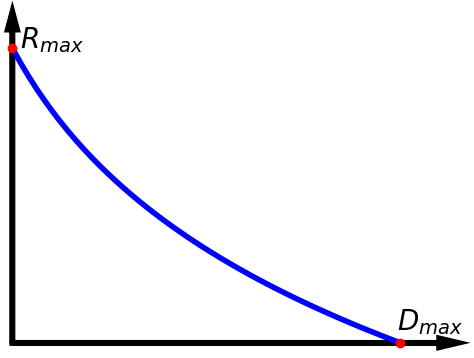
\includegraphics[width=0.26\textwidth]{RD_II/RD_Plot_Final.png}
\captionsetup{labelformat=empty}
%\caption{Illustration of convexity.}
\end{figure}
\end{frame}




\subsection{Review of last lecture}

\begin{frame}
 \vspace{12.0ex}
\begin{center}
\begin{beamercolorbox}[sep=12pt,center]{part title}
\usebeamerfont{section title}\insertsubsection\par
\end{beamercolorbox}
\end{center}
\end{frame}

\begin{frame}{Lossy source codes. Rate and distortion.}
Given discrete random variable $X$ with values in some $\mathbb{R}^N$ with finite alphabet $\mathcal{A}_X$ and distribution $p_{X}$. 
%\vspace{-0.03cm}

\loud{Lossy source codes} $Q=(\alpha,\gamma,\beta)$:
\bit
\item $\alpha: \mathcal{A}_X\to \mathcal{I}_K:=\{1,\dots,K\}$, \loud{quantization}
\item $\gamma$: \loud{Lossless mapping}. Uniquely decodable code for $\mathcal{I}_K$. 
\item $\beta: \mathcal{I}_K\to\widehat{\mathcal{A}}$, \loud{inverse quantization}. Set $\widehat{\mathcal{A}}\subset\mathbb{R}^N$ is called \loud{reproduction alphabet}. 
\item In general: $\beta(\alpha(x))\neq x$. Information can not be recovered exactly by decoder.
%\item Rate and distortion 
\eit
\loud{Rate and distortion of $Q$:}
\bit
\item \loud{Rate $r(Q)$:} Expected length of codewords $\gamma(\alpha(x))$ with $x\in\mathcal{A}$:  
\begin{align*}
r(Q):=\sum_{\mathbf{x}\in\mathcal{A}}p_X(x)\ell(\gamma(\alpha(x)).
\end{align*}
\item \loud{Distortion $\delta(Q)$:} Expected 
 deviation of original and reconstructed symbols measured with a given \loud{distortion function} $d$:
\begin{align*}
\delta(Q):=\sum_{\mathbf{x}\in\mathcal{A}}p_X(x)d(x,\beta(\alpha(x))).
\end{align*}
\eit
\end{frame}



\begin{frame}{Fundamental task of lossy source coding. Rate distortion function.}
\loud{Fundamental task of lossy source coding:}
\bit
\item []For a maximal allowable distortion $D$, find a source code $Q$ of rate $r(Q)$ as small 
as possible such that $\delta(Q)\leq D$. 
\eit 

\loud{Rate distortion function: }
\bit
\item Quantifies how good the above task can be solved at all. For $D\in [0,\infty)$, one puts
\begin{align*}
R(D)= \inf\{r(Q)\colon \text{$Q$ is a source code with $\delta(Q)\leq D$}\}.
\end{align*}
\item For $D=0$, lossless scenario: 
\bit
\item Can bound $R(0)$ in terms of \loud{entropy} of the source $X$. 
\item \loud{Huffman coding}: Explicit construction of optimal source code.  
\eit 
\eit 
\loud{\iarrow$ $ Goal: Describe $R(D)$ also for $D>0$. Fundamental theorem of lossy source coding.} 
\end{frame}


\begin{frame}{Mutual information. Informational rate distortion function.}
\loud{Mutual information for random variables $X$ and $Y$:}
\bit
\item Reduction of uncertainty of $X$ given $Y$:
\[
I(X;Y)=H(X)-H(X|Y).
\]
\item Mutual information is symmetric, nonnegative, zero if and only if $X$ and $Y$ are independent. 
\item Analogous definition of $I(p;q)$ for pmf $p=p_X$ with alphabet $\mathcal{A}$ and conditional pmf $q(\cdot|x)$, $x\in\mathcal{A}$ on 
alphabet $\mathcal{B}$. 
\eit
\loud{Informational rate-distortion functio}n
\bit
\item The informational rate-distortion function is defined as 
\begin{align}\label{DefInfRDRProb}
R^{(I)}(D):=\inf\{I(p_X;q)\colon \sum_{x\in\mathcal{A}}\sum_{\hat{x}\in\mathcal{B}}q(\hat{x}|x)p_X(x)d(x,\hat{x})<D\}
\end{align}
\item In \eqref{DefInfRDRProb}, $q$ is taken over the set of all conditional probabilities $q(\cdot|x)$ with finite alphabet $\mathcal{B}$.
\item Last lecture: \loud{Entropy is concave \iarrow $R^{(I)}$ is convex.} 
\eit
\end{frame}

\begin{frame}{Joint coding of independent realizations of a source}
Let $X$ be an $\mathbb{R}$-valued random variable.
 
\loud{Independent realizations of $X$. Joint coding}
\bit
\item For each $N\in\mathbb{N}$ let $X^N=(X_1,\dots,X_N)$ be $\mathbb{R}^N$-valued random variable with \loud{$N$ independent realizations} $X_i$ of $X$.
\item For each $i$, one has 
$p_{X_i}=p_{X}$.
\item Joint distribution $p_{X^N}$ of $(X_1,\dots,X_N)$ 
satisfies
\begin{align}\label{DefJointI}
p_{X^N}(x_1,\dots,x_N)=p^{\times N}(x_1,\dots,x_N):=p^{\times N}_X(x_1,\dots,x_N):=p_{X}(x_1)\cdot \cdots \cdot p_{X}(x_N). 
\end{align}
\item Precise computation of rate-distortion function only possible for $X^N$ with $N\to\infty$.
\item Source codes for $X^N$ with rate distortion performance close to value of rate distortion function are usually \textit{not} $N$ realizations of source codes for $X$. 
\item Main reason: Vector quantization advantage. 
\eit
\end{frame}


\begin{frame}{The fundamental theorem of lossy source coding}
\begin{theorem}[Fundamental theorem of lossy source coding]
Let $X$ be a discrete $\mathbb{R}$-valued random variable. Fix an additive distortion measure. 
\begin{enumerate}
\item The informational rate distortion function $R^{I}$ is always a \loud{lower bound} for the rate distortion function: 
For every $N\in\mathbb{N}$ and every sorce code $Q_N$ for $X^N$ one has  
\begin{align}\label{BoundRate}
r(Q_N)\geq R^{(I)}(\delta(Q_N)). 
\end{align}
\item The bound \eqref{BoundRate} is \loud{asymptotically achievable}:

For every $D>0$, every $\epsilon>0$ and every $R'>R^{(I)}(D)$,  there exists a sequence 
of source codes $Q_N$ with $N\to\infty$ such that for all $N$ sufficiently large one has 
\begin{align*}
\delta(Q_N)\leq D+\epsilon
\end{align*}
and such that
\begin{align*}
r(Q_{N})\leq R'. 
\end{align*}
\end{enumerate}
\end{theorem}
\end{frame}

\subsection{Informational rate distortion function is lower bound for rate distortion function}
\begin{frame}
 \vspace{8.0ex}
\begin{center}
\begin{beamercolorbox}[sep=12pt,center]{part title}
\usebeamerfont{section title}\insertsubsection\par
\end{beamercolorbox}
\end{center}
\end{frame}
%\subsubsection{Convexity of the informational rate distortion function}
%\begin{frame}{Review: Convexity and concavity}
%\loud{Recall: Convexity of a function}
%\bit
%\item A function $f:(a,b)\to\mathbb{R}$ is called \loud{convex} if for any two point $p_1,\:p_2\in (a,b)$, the straight
%line between $(p_1, f(p_1))$ and $(p_2, f(p_2))$ lies above the graph of $f$:
%\begin{align}\label{eqconv}
%f((1-\lambda)p_1+\lambda p_2)\leq (1-\lambda)f(p_1)+\lambda f(p_2), \quad \forall \lambda\in [0,1] 
%\end{align}  
%\item  $f$ is called \loud{strictly convex} if strict inequality holds in \eqref{eqconv} for all $\lambda\in (0,1)$ and 
%all $p_1\neq p_2$. 
%\item $f$ is calleld (strictly) \loud{concave}, if $-f$ is (strictly) convex. 
%\eit
%\begin{figure}
%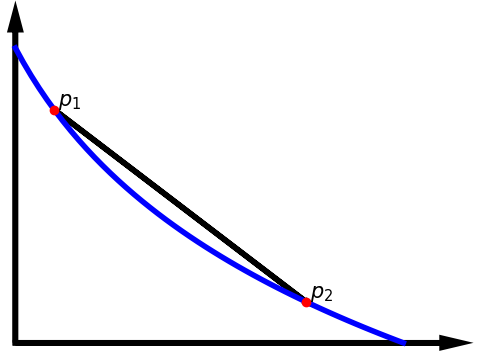
\includegraphics[width=0.26\textwidth]{RD_Plot_Convex_Final.png}
%\captionsetup{labelformat=empty}
%\caption{Illustration of convexity.}
%\end{figure}
%\end{frame}
%
%\begin{frame}{Elementary properties of convex functions}
%\loud{Jensen's inequality}
%\bit
%\item If $f$ is convex on $(a,b)$, then for all $\lambda_1,\dots,\lambda_n\in[0,1]$ with $\lambda_1+\dots+\lambda_n=1$ and all 
%$p_1,\dots,p_n\in (a,b)$, one has
%\begin{align*}
%f(\lambda_1 p_1+\dots+\lambda_np_n)\leq \lambda_1f(p_1)+\dots+\lambda_nf(p_n). 
%\end{align*}
%\item If $f$ is strictly convex and all $p_i$ different, equality only if $\lambda_i=1$ for an $i\in\{1,\dots,n\}$. 
%\item Proof by induction.
%\eit
%\loud{Characterization for continuously differentiable functions}
%\bit
%\item If $f$ is continously differentiable, then $f$ is (strictly) convex if and only if $f'$ is (strictly) monotonically increasing. 
%\item Analogous statement for concave functions.  
%\item Proof: Application of  mean value theorem of differential calculus.
%\eit
%
%
%\end{frame}
%
%\begin{frame}{Concavity of entropy}
%\begin{proposition}[Concavity of entropy]
%Let $p_1$, $p_2$ be probability mass functions on a finite alphabet $\mathcal{A}$. 
%Then for every $\lambda\in(0,1)$ one has 
%\begin{align*}
%H((1-\lambda)p_1+\lambda p_2)\geq (1-\lambda)H(p_1)+\lambda H(p_2), \quad \text{equality if an only if $p_1=p_2$}. 
%\end{align*}
%\end{proposition}
%%\vspace{-0.1cm}
%%\small Heuristic explanation: Averaging two pmfs gives a `more equidistributed pmf' $\iarrow$ entropy increases. 
%\vspace{-2.9mm}
%%\smallskip
%\loud{Proof: } 
%%\vspace{-1.5mm}
%\bit 
%\item Let $f(t):=-t\log_2(t)$. 
%\item The derivative $f'(t)=-\frac{1}{\ln(2)}(1+\ln(t))$ is strictly decreasing $\loud\iarrow$ f is strictly concave. 
%\item[\iarrow] By definition of the entropy:
%\begin{align*}
%H((1-\lambda)p_1+\lambda p_2)=\sum_{a\in\mathcal{A}}f((1-\lambda)p_1(a)+\lambda p_2(a))
%\geq & \sum_{a\in\mathcal{A}}\left((1-\lambda)f(p_1(a))+\lambda f(p_2(a))\right)\\
%=&(1-\lambda)H(p_1)+\lambda H(p_2).
%\end{align*} 
% \item Statement of equality follows from strict concavity of $f$.  \qed
%\eit
%Heuristic explanation: Averaging two pmfs gives a `more equidistributed pmf' $\iarrow$ entropy increases. 
%\end{frame}
%
%
%
%
%\begin{frame}{Convexity of the informational rate distortion function}
%\begin{proposition}[Convexity of $R^{(I)}$]
%The informational rate distortion function $R^{(I)}$ is convex.
%\end{proposition}
%\vspace{-2.9mm}
%\loud{Proof: } 
%%\vspace{-1.0mm}
%\bit
%\item \loud{Main idea:} Use concavity of entropy, i.e. convexity of negative entropy. 
%\item Let $\lambda\in [0,1]$ and $D_1,\:D_2\in[0,\infty)$. %One needs to show that
%%\[
%%R^{(I)}((1-\lambda)D_1+\lambda D_2)\leq (1-\lambda)R_I(D_1)+\lambda R(D_2). 
%%\]
%%
%%
%\item Let $q_1$ and $q_2$ be any conditional probabilities with alphabets $\mathcal{B}_1$ and $\mathcal{B}_2$ such that
%\begin{align}\label{DistConstrIndiv}
%\sum_{x\in\mathcal{A}}\sum_{\hat{x}\in\mathcal{B}_1}p(x)q_1(\hat{x}|x)d(x,\hat{x})<D_1; \quad \sum_{x\in\mathcal{A}}\sum_{\hat{x}\in\mathcal{B}_2}p(x)q_2(\hat{x}|x)d(x,\hat{x})<D_2.
%\end{align}
%
%\item Define a conditional probability $q_3$ with alphabet $\mathcal{B}=\mathcal{B}_1\cup\mathcal{B}_2$ as 
%\begin{align*}
%q_3=(1-\lambda)p_1+\lambda p_2
%\end{align*}
%\item By \eqref{DistConstrIndiv}, putting $p=p_X$, $q_3$ satisfies the distortion constraint
%\begin{align}\label{DistConstrQ3}
%\sum_{x\in\mathcal{A}}p(x)\sum_{\hat{x}\in\mathcal{B}}q_3(\hat{x}|x)d(x,\hat{x}) \leq (1-\lambda)D_1+\lambda D_2. 
%\end{align}
%\eit
%\end{frame}
%
%
%\begin{frame}{Proof of the convexity of $R^{(I)}$}
%\bit
%\item By the concavity of entropy: 
%\begin{align*}
%-H(q_3|p)=-\sum_{x\in\mathcal{A}}p(x)H(q_3(\cdot|x))\leq& -\sum_{x\in\mathcal{A}}p(x)\left((1-\lambda)H(q_1(\cdot|x))+\lambda H(q_2(\cdot|x))\right)\\
%=&-(1-\lambda)H(q_3|p)-\lambda H(q_3|p)
%\end{align*}
%\item [\iarrow] Using definition of $R^{(I)}$ and \eqref{DistConstrQ3}:
%\begin{align}\label{estD}
%R^{(I)}((1-\lambda)D_1+\lambda D_2)\leq I(p;q_3)=H(p)-H(p|q_3)\leq &(1-\lambda)H(p)+H(p|q_1)+\lambda( H(p)+H(p|q_2)) \nonumber\\ =&(1-\lambda)I(p;q_1)+\lambda I(p;q_2).
%\end{align}
%\item Now use:
%\bit
%\item $q_1$ and $q_2$ were arbitrary conditional probabilities satisfying \eqref{DistConstrIndiv}. 
%\item Infimum of linear combinations is linear combination of infima. 
%\item Infimum is largest lower bound. 
%\eit
%\item[\iarrow] It follows from \eqref{estD} that
%\begin{align*}
%R^{(I)}((1-\lambda)D_1+\lambda D_2)\leq (1-\lambda)R^{(I)}(D_1)+\lambda R^{(I)}(D_2). 
%\end{align*}
%\qed
%\eit 
%\end{frame}
%
%

\subsubsection{Lower bound of rate by mutual informations}

\begin{frame}{Lower bound for rate by mutual informations I}
\begin{proposition}[Estimate of rate by mutual informations]
Let $Q=(\alpha,\gamma,\beta)$ be a source code for $X^N$. 
Let $Y:=\beta(\alpha(X^N))$ with $Y=(Y_1,\dots,Y_N)$.
Then one has 
\begin{align}\label{EqRateSumMut}
r(Q)\geq (1/N)\sum_{i=1}^{N}I(X_i,Y_i).
\end{align}
\end{proposition}
\loud{Proof:}
\bit 
\item The encoder needs to transmit $\alpha(X^N)$. \loud{Entropy is lower bound for rate } and $r$ is rate per symbol:
\begin{align*}
r(Q)\geq (1/N)H(\alpha(X^N)).
\end{align*}
\item Since $\alpha(X^N)$ determines $Y$, by the \loud{data processing inequality} one has 
\begin{align*}
H(\alpha(X^N))\geq H(Y).
\end{align*}
\item Since $X^N$ determines $Y$, one has $H(Y|X^N)=0$.  Using the symmetry of $I$, it follows that
\begin{align*}
H(Y)=H(Y)-H(Y|X^N)=I(Y;X^N)=I(X^N;Y)=H(X^N)-H(X^N|Y).
\end{align*}
\eit 
\end{frame}


\begin{frame}{Lower bound for rate by mutual informations II}
\bit
%\item Since $\mathbf{X}$ determines $\mathbf{Y}$, one has $H(\mathbf{Y}|X^N)=0$ by the data processing inequality.  Using the symmetry of $I$, it follows that
%\begin{align*}
%H(\mathbf{Y})=H(\mathbf{Y})-H(\mathbf{Y}|X^N)=I(\mathbf{Y};X^N)=I(X^N;\mathbf{Y})=H(X^N)-H(X^N|\mathbf{Y}).
%\end{align*}
%\item Since $\mathbf{Y}$ determines $Y_i$ via the projection onto the $i$-th coordinate, it follows that
%\begin{align*}
%H(X_i|\mathbf{Y})\leq H(\mathbf{X}|Y_i). 
%\end{align*}
%By the chain rule, one has 
%%\begin{align*}
%%H(\mathbf{X}|Y_i)=\sum_
%%\end{align*}
\item Since $X^N$ is iid, one has
\begin{align*}
H(X^N)=\sum_{i=1}^NH(X_i).
\end{align*}
\item By the chain-rule, one has
\begin{align*}
H(X^N|Y)=\sum_{i=1}^NH(X_i|Y,X_1,\dots,X_{i-1}).
\end{align*}
\item Since $(Y,X_1,\dots,X_{i-1})$ determines $Y_i$ (or since ``conditioning does not increase entropy'') one has
\begin{align*}
H(X_i|Y,X_1,\dots,X_{i-1})\leq H(X_i|Y_i).  
\end{align*}
\item Combining all above items gives
\begin{align*}
r(Q)\geq (1/N) \sum_{i=1}^N(H(X_i)-H(X_i|Y_i))=(1/N) \sum_{i=1}^NI(X_i,Y_i). \qed
\end{align*}
\eit 
\end{frame}

\subsubsection{Completion of the proof}
\begin{frame}{Completion of the proof I}
\loud{Idea: Use previous proposition and convexity of $R^{(I)}$}.
\bit
\item Let $Q=(\alpha,\beta,\gamma)$ be a source code for $X^N$.
\item Let $Y$ and $Y_i$ be as in previous proposition and let $p_{X_i,Y_i}$ be the joint distribution of $X_i$ and $Y_i$.
\item Let 
\begin{align*}
\delta_i:=\sum_{(x,y)\in\mathcal{A}\times\hat{\mathcal{A}}}p_{X_i,Y_i}(x,y)d(x,y)
\end{align*}
be the expected distortion between $X_i$ and $Y_i$. 
\item By \eqref{EqRateSumMut} and by the definition of $R^{(I)}$, one has 
\begin{align}\label{VorletzteGlr}
r(Q)\geq &
(1/N) \sum_{i=1}^NI(X_i;Y_i)\nonumber\\ \geq &(1/N)\sum_{i=1}^NR^{(I)}(\delta_i).
\end{align}
\eit 
\end{frame}


\begin{frame}{Completion of the proof II}

\bit
\item For $x\in\mathcal{A}$, $y\in\widehat{\mathcal{A}}$, joint distribution $p_{X_i,Y_i}$ satisfies
\begin{align*}
p_{X_i,Y_i}(x,y)=p_X^{\times N}(\mathbf{x}=(x_1,\dots,x_i,\dots,x_N)\in\mathcal{A}^N\colon Y_i(\mathbf{x})=y\text{ and $x_i=x$}).%,\quad x\in\mathcal{A}, \quad y\in\widehat{\mathcal{A}}.
\end{align*}
\item Since distortion function is additive, 
if $\beta_i$ denotes the $i$-th component of $\beta$, it follows that 
\begin{align*}
\delta(Q)=&(1/N)\sum_{\mathbf{x}\in\mathcal{A}^N}p_X^{\times N}(\mathbf{x})\sum_{i=1}^Nd(x_i,\beta_i(\alpha(\mathbf{x})))=(1/N)\sum_{i=1}^N\delta_i. 
\end{align*} 
\item By \eqref{VorletzteGlr} and the \loud{convexity of $R^{(I)}$} [last lecture!], it follows that
\begin{align*}%\label{LetzteGlr}
r(Q)\geq (1/N)\sum_{i=1}^NR^{(I)}(\delta_i)\geq & R^{(I)}\biggl((1/N)\sum_{i=1}^N\delta_i\biggr)\\ =&R^{(I)}(\delta(Q)).
\end{align*}
\qed
\eit
\end{frame}


%\begin{frame}{Estimate of rate by mutual informations}
%\bit
%\item Since $\mathbf{X}$ is iid, $X_i\sim X$, one has
%\begin{align*}
%H(\mathbf{X})=\sum_{i=1}^nH(X_i)
%\end{align*}
%\item By the chain-rule, one has
%\begin{align*}
%H(\mathbf{X}|\mathbf{Y})=\sum_{i=1}^NH(X_i|\mathbf{Y},X_1,\dots,X_i).
%\end{align*}
%\item Since $(\mathbf{Y},X_1,\dots,X_i)$ determines $Y_i$ (or since ``conditioniong does not increase entropy'') one has
%\begin{align*}
%H(X_i|\mathbf{Y},X_1,\dots,X_i)\leq H(X_i|Y_i).  
%\end{align*}
%\item Combining the chain of inequlities gives 
%\begin{align*}
%R\geq \sum_{i=1}^nH(X_i)-H(X_i|Y_i)=\sum_{i=1}^nI(X_i|Y_i). \qed
%\end{align*}
%\eit 
%\end{frame}
%
%\begin{frame}
%\bit 
%\item \loud{Idea: Use convexity of $R^{(I)}$ and previous proposition}.
%\item \loud{Property of joint distributions $p_{X_i,Y_i}$}: 
%
%For all $x,\hat{x}\in\mathcal{A}$ and all $i\in\{1,\dots,N\}$,  $p_{X_i,Y_i}(x,\hat{x})$ is equal to the probability $p^{\times N}$ 
%of all $\mathbf{x}=(x_1,\dots, x_{i-1},x_i,x_{i+1},\dots,x_N)\in\mathcal{A}^N$ 
%with $x_i=x$ and $g_i(f(\mathbf{x}))=\hat{x}$. 
%\item Consequece: One has
%\begin{align*}
%D_i:=\sum_{x\in\mathcal{A}}\sum_{\hat{x}\in\mathcal{A}}p_{X_i,Y_i}(x,\hat{x})d(x,\hat{x})
%%=&\sum_{x\in\mathcal{A}}\sum_{\hat{x}\in\mathcal{A}}p_{Y_i|X_i}(\hat{x}|x)d(x,\hat{x})\\
%%\]
%%\item It easily follows from the definition that
%%then 
%%\[
%%D_i
%=&\sum_{\mathbf{x}=(x_1,\dots,x_N)\in\mathcal{A}^N}p^{\times N}(\mathbf{x})d(x_i,g_i(f(\mathbf{x}))).
%\end{align*}
%\item Thus, using ..., it follows that 
%\begin{align*}
%D=\sum_{\mathbf{x}\in\mathcal{A}^N}p^{\times N}(\mathbf{x})d_N(\mathbf{x},\mathbf{Y}(\mathbf{x}))
%=&\sum_{\mathbf{x}=(x_1,\dots,x_N)\in\mathcal{A}^N}p^{\times N}(\mathbf{x})(d(x_1,Y_1(\mathbf{x}))+\cdots+d(x_N,Y_N(\mathbf{x}))
%\\=&\sum_{i=1}^N D_i.
%\end{align*}
%\item[\iarrow] Using \eqref{EqRate} and the convexity of $R^{(I)}$, it follows that
%\begin{align*}
%R\geq \sum_{i=1}^NI(X_i;Y_i)\geq \sum_{i=1}^NR^{(I)}(D_i)\geq R^{I}(D)\qed 
%\end{align*}
%\eit
%\end{frame}







\subsection{Proof of asymptotic achievability}
\begin{frame}
 \vspace{8.0ex}
\begin{center}
\begin{beamercolorbox}[sep=12pt,center]{part title}
\usebeamerfont{section title}\insertsubsection\par
\end{beamercolorbox}
\end{center}
\end{frame}

\subsubsection{Setup for the proof} 
\begin{frame}{Setup for the proof}
\bit
\item Let $D>0$, $\epsilon>0$ and $R'>R^{(I)}(D)$ be as in the fundamental theorem of lossy source coding.
\item Can assume that $\epsilon$ is so small that $R'>R^{(I)}(D)+3\epsilon/2$.
\item Let $q$ be a conditional probability on $\hat{\mathcal{A}}$ which satisfies the distortion constraint
\begin{align*}
\sum_{x\in\mathcal{A}}\sum_{\hat{x}\in\hat{\mathcal{A}}}q(\hat{x}|x)p_X(x)d(x,\hat{x})<D. 
\end{align*}
from \eqref{DefInfRDRProb} and for which
$I(p;q)<R'$. 
\item Marginal $p_X$ and conditional $q$ define a joint distribution on $\mathcal{A}\times\hat{\mathcal{A}}$
\item Realize this joint distribution as distribution $p_{X,\hat{X}}$ of  
an $\mathcal{A}\times\hat{\mathcal{A}}$-valued random variable $(X,\hat{X})$. 
\item Define $p_{\hat{X}}^{\times N}$ on ${\hat{\mathcal{A}}}^N$ and  $p_{X,\hat{X}}^{\times N}$ on 
$\mathcal{A}^N\times\hat{{\mathcal{A}}}^N$ by
\begin{align}\label{DefJointII}
p_{\hat{X}}^{\times N}(\hat{x}_1,\dots,\hat{x}_N)=&p_{\hat{X}}(\hat{x}_1)\cdot \cdots\cdot p_{\hat{X}}(\hat{x}_N)\nonumber;
\\ p_{X\times\hat{X}}^{\times N}((x_1,\dots,x_N),(\hat{x}_1,\dots,\hat{x}_N))=&p_{X\times\hat{X}}(x_1,\hat{x}_1)\cdot \cdots\cdot p_{X\times\hat{X}}(x_N,\hat{x}_N).
\end{align}
\item Can assume that $R'$ is a rational number. Choose all $N$ such that $NR'$ is an integer.
\eit
\end{frame} 


\subsubsection{The ensemble set and typical sequences}
\begin{frame}{Definition of the ensemble set and random coding}
\loud{The ensemble set $\mathcal{E}_N$:}
\bit
\item The set of all $\hat{\mathcal{A}}^N$-valued sequences of length $2^{NR'}$: 
\[
\mathcal{E}_N:=\{\mathcal{C}=({\hat{\mathbf{x}}}_1,\dots,{\hat{\mathbf{x}}}_{2^{NR'}})\colon {\hat{\mathbf{x}}}_i\in{\hat{\mathcal{A}}}^N\}.
\]
%\item Each $\mathcal{C}\in\mathcal{E}_N$ is called a \loud{codebook}. 
\item $\mathcal{E}_N$ is a discrete propability space, probability $P_{\mathcal{E}_N}$ defined as
\begin{align}\label{ProbEnsemble}
P_{\mathcal{E}_N}(({\hat{\mathbf{x}}}_1,\dots,{\hat{\mathbf{x}}}_{2^{NR'}}))=p_{\hat{X}}^{\times N}({\hat{\mathbf{x}}}_1)\cdot \cdots \cdot p_{\hat{X}}^{\times N}({\hat{\mathbf{x}}}_{2^{NR'}}).
\end{align}
\item Using \loud{typical sequences}, each $\mathcal{C}=({\hat{\mathbf{x}}}_1,\dots,{\hat{\mathbf{x}}}_{2^{NR'}})\in\mathcal{E}_N$ defines a lossy source code for $\mathcal{A}^N$ of rate $R'$ bits per symbol.  
%\item Use \loud{typical sequences} for the definition of the source codes, see below.
\item[\iarrow] \loud{Random coding:} Ensemble set is a probability space of source codes. 
\eit

\end{frame}


\begin{frame}{Typical sequences}
\loud{The set of typical sequences $A_{d, \epsilon}^{(N)}$}:
\bit
\item Let $A_{d, \epsilon}^{(N)}$ be the set of all pairs 
$(\mathbf{x},\hat{\mathbf{x}})\in\mathcal{A}^N\times{\hat{\mathcal{A}}}^N$ 
such that the following four conditions hold. 
\small
\begin{align}
\left|-\frac{1}{N}\log_2(p_X^{\times N}(\mathbf{x}))-H(X)\right|<\epsilon/2\label{FirstEqEntrTyp}\\
\left|-\frac{1}{N}\log_2(p_{\hat{X}}^{\times N}(\hat{\mathbf{x}}))-H(\hat{X})\right|<\epsilon/2\label{SecondEqEntrTyp}\\
\left|-\frac{1}{N}\log_2(p_{X,\hat{X}}^{\times N}(\mathbf{x},\hat{\mathbf{x}}))-H(X,\hat{X}))\right|<\epsilon/2\label{ThirdEqEntrTyp}\\
\left|d_N(\mathbf{x},\hat{\mathbf{x}})-D\right|<\epsilon/2\label{EqDistTypical}.
\end{align}
\normalsize
%
%
%\bit
%\item $\left|-\frac{1}{N}\log_2(p_X^{\times N}(\mathbf{x}))-H(X)\right|<\epsilon$
%\item $\left|-\frac{1}{N}\log_2(p_{\hat{X}}^{\times N}(\hat{\mathbf{x}}))-H(\hat{X})\right|<\epsilon$
%\item $\left|-\frac{1}{N}\log_2(p_{X,\hat{X}}^{\times N}(\mathbf{x},\hat{\mathbf{x}}))-H(X,\hat{X}))\right|<\epsilon$
%\item $\left|\log_2(d_N(\mathbf{x},\hat{\mathbf{x}}))-\mathbb{E}(d(X,\hat{X}))\right|<\epsilon$
%\eit
\item Apply \loud{law of large numbers}, reviewed below, to the random variables $\log_2(p_X)$, $\log_2(p_{\hat{X}})$, $\log_2(p_{X,\hat{X}})$, $d(X,\hat{X})$ and use 
\eqref{DefJointI}, \eqref{DefJointII} and that $d_N$ is additive extension of $d$: 
\item[\iarrow] For every $\epsilon>0$, one has 
\begin{align}\label{ProbTypicalSet}
\lim_{N\to\infty} p_{X,\hat{X}}^{\times N}\bigl(A_{d, \epsilon}^{(N)}\bigr)=1. 
\end{align}
\eit 

\end{frame}


\begin{frame}{Ensemble set as a set of source codes} 
\loud{Each $\mathcal{C}\in\mathcal{E}_N$ defines a source-code for $\mathcal{A}^N$:}
\bit
\item[] \loud{Quantization $\alpha$:}
\bit
\item For $\mathcal{C}=({\hat{\mathbf{x}}}_1,\dots,{\hat{\mathbf{x}}}_{2^{NR'}})$ and $\mathbf{x}\in\mathcal{A}^N$ let 
$\mathsf{i}=\alpha(\mathbf{x})$ be the smallest $\mathsf{i}\in\{1,\dots,2^{NR'}\}$ such that 
\begin{align*}
(\mathbf{x},{\hat{\mathbf{x}}}_{\mathsf{i}})\in A_{d,\epsilon}^{(N)}, 
\end{align*}
if such an $\mathsf{i}$ exists. If such an $\mathsf{i}$ does not exist, put $\mathsf{i}=1$. 
\eit
\item[] \loud{Lossless mapping $\gamma$:}
\bit 
\item Fixed length code: Each $i\in\{1,\dots,2^{NR'}\}$ is mapped to its binary representation of $NR'$ bits. 
\eit 
\item[] \loud{Inverse quantization $\beta$:}
\bit 
\item Map a given $i\in\{1,\dots,2^{NR'}\}$ to the element ${\hat{\mathbf{x}}}_i\in{\hat{\mathcal{A}}}^N$. 
\eit
%\item For $\mathbf{x}\in\mathcal{A}^N$ write $\mathcal{C}(x)\in\widehat{\mathcal{A}}^N$ for the corresponding decoded symbol, i. e. 
%$\mathcal{C}(x)=\beta(\alpha(\mathbf{x}))$.  
\eit
\bit
\item[\iarrow] \loud{Rate of all source codes $\mathcal{C}\in\mathcal{E}_N$ is  $NR'$, i.e. $R'$ bits per symbol. }
\item[\iarrow]\loud{What about the distortion?} 
\item[\iarrow]\loud{Key idea: } Show that \loud{expectation value of the distortion over $\mathcal{E}_N$} is smaller than $D+\epsilon$.
\eit
\end{frame}

\subsubsection{Review of law of large numbers}

\begin{frame}{Review: Law of large numbers}
Let $(\Omega,P)$ be a discrete probability space.
\bit
\item A sequence $(X_i)_{i=1}^\infty$ of random variables is called \loud{independent identically distributed (iid)} if 
\bit
\item $p_{X_{i_1},\dots,X_{i_k}}=p_{X_{i_1}}\cdot \cdots \cdot p_{X_{i_k}} $ for all indices $1\leq i_1<\dots<i_k$
\item $p_{X_i}=p_{X_j}$ for all $i$ and $j$. 
\eit
\item  If $(X_i)_{i=1}^\infty$ is iid, all expectation values
\[
\mathbb{E}(X_i)=\sum_{x\in\mathcal{A}_{X_i}}p_{X_i}(x)\cdot x.
\]
are equal.   
\item \loud{\textbf{Law of large numbers}} (weak form): If $(X_i)_{i=1}^\infty$ is \textbf{iid}, then the \textbf{sequence 
of averages} of the $X_i$ \textbf{converges} in probability \textbf{to the expectation value} $\mathbb{E}(X_i)=a$.
For every $\epsilon>0$, one has 
\[
\lim_{N\to\infty}P\left(\left|\frac{1}{N}\sum_{i=1}^NX_i-a\right|>\epsilon\right)=0. 
\]
\eit 
\end{frame}

\begin{frame}{Law of large numbers: Example and comments}
\loud{Example for theorem of large numbers: }
\bit
\item Throwing a dice gives probability mass function $\mu$ with $\mu(1)=\mu(2)=\dots=\mu(6)=1/6$ on $\mathbb{R}$.
\item By Kolmogorov's extension theorem: There exists a probability
space $\Omega$ and iid. random-variables $(X_i)_{i=1}^\infty$ on $\Omega$ such that $p_{X_i}=\mu$ for all $i$. 
\item Can interpret $X_i$ as independent trials of throwing a dice at time instances $i$.
\item[\iarrow] Law of large numbers: If one performs $N$ independent trials of throwing a dice,  average value of outcomes approaches $3.5$ arbitrary close with an arbitrary high probability as $N\to\infty$. 
\eit 
\loud{Extensions:} 
\bit
\item Strong law of large numbers: The sequence of averages in fact converges allmost surely to $\mathbb{E}(X_i)$. This means that the probability of all $\omega\in\Omega$ where 
it does not converge is zero. Not needed here. 
\item Weak and strong law of large numbers also hold for continuous probability spaces and random variables, if expectation value is finite.
\eit
\end{frame}



\subsubsection{Expected distortion over the ensemble set}
\begin{frame}{Expected distortion over the ensemble set}
Expected distortion over $\mathcal{E}_N$ with respect to $P_{\mathcal{E}_N}$ is 
\begin{align*}%\label{ExpectedDist}
\mathbb{E}_{P_{\mathcal{E}_N}}(\delta_N(\cdot))=\sum_{\mathcal{C}\in\mathcal{E}_N}P_{\mathcal{E}_N}(\mathcal{C})\delta_N(\mathcal{C}).
\end{align*}

\bit
\item Each $\delta_N(\mathcal{C})$ is an expectation value over $\mathcal{A}^N$.
\item [\iarrow] Expected distortion over $\mathcal{E}_N$ is an expectation value of expectation values.
\item By \eqref{EqDistTypical}, for all $(\mathbf{x},\hat{\mathbf{x}})\in A_{d,\epsilon}^{(N)}$, one can estimate
\begin{align}\label{EstDistTypical}
d_N(\mathbf{x},\hat{\mathbf{x}})<D+\epsilon/2.
\end{align}
\item Since $\mathcal{A}$ and $\hat{\mathcal{A}}$ are finite, there exists a $D_{max}\in (0,\infty)$ such that for all $\mathbf{x}\in\mathcal{A}^N$ and all $\hat{\mathbf{x}}\in{\hat{\mathcal{A}}}^N$ one can 
estimate
\begin{align}\label{EstDistAlways}
d_N(\mathbf{x},\hat{\mathbf{x}})<D_{max}.
\end{align}
\eit
\end{frame}



\begin{frame}{Bounding the expected distortion over the ensemble set}
\loud{Idea:} 
\bit
\item Split $\mathbb{E}_{P_{\mathcal{E}_N}}(\delta_N(\cdot))$ into contributions from $A_{d,\epsilon}^{(N)}$ and from complement of $A_{d,\epsilon}^{(N)}$ . 
\item On $A_{d,\epsilon}^{(N)}$, distortion behaves as expected. 
\item Bound contribution from complement of $A_{d,\epsilon}^{(N)}$ invoking the mutual information $I(X;\hat{X})$. 
\eit 

\loud{Bounding contribution from non-typical sequences:} 
\bit
\item For $\mathbf{x}\in\mathcal{A}^N$ write $\mathcal{C}(x)\in\widehat{\mathcal{A}}^N$ for the corresponding decoded symbol, i. e. 
$\mathcal{C}(x)=\beta(\alpha(\mathbf{x}))$.  
\item For every $\mathbf{x}\in\mathcal{A}^N$ let 
\begin{align*}
P_e(\mathbf{x})=\sum_{\mathcal{C}\in\mathcal{E}_N\colon (\mathbf{x},C(\mathbf{x}))\notin A_{d,\epsilon}^{(N)}}P_{\mathcal{E}_N}(\mathcal{C}).
\end{align*}
\item $P_e(\mathbf{x})$ is the probability of all sequences $\mathcal{C}\in\mathcal{E}_N$ which do \textit{not} contain 
an ${\hat{\mathbf{x}}}_i$ with $(\mathbf{x},{\hat{\mathbf{x}}}_i)\in A_{d, \epsilon}^{(N)}$.
\eit

\end{frame}



\begin{frame}{Bounding expected distortion over the ensemble set in terms of probability $P_e(\mathbf{x})$}
\bit
\item Applying \eqref{EstDistTypical} and \eqref{EstDistAlways}, one can estimate 
\small
\begin{align}\label{EstimateByPE}
\mathbb{E}_{P_{\mathcal{E}_N}}(\delta_N(\cdot))=& \sum_{\mathcal{C}\in\mathcal{E}_N}P_{\mathcal{E}_N}(\mathcal{C})\sum_{\mathbf{x}\in\mathcal{A}^N}p^{\times N}_X(\mathbf{x})d_N(\mathbf{x},\mathcal{C}(\mathbf{x}))\nonumber\\
=&\sum_{\mathcal{C}\in\mathcal{E}_N}P_{\mathcal{E}_N}(\mathcal{C})\sum_{\mathbf{x}\colon (\mathbf{x},C(\mathbf{x}))\in A_{d,\epsilon}^{(N)}}p^{\times N}_X(\mathbf{x})d_N(\mathbf{x},\mathcal{C}(\mathbf{x}))
+\sum_{\mathcal{C}\in\mathcal{E}_N}P_{\mathcal{E}_N}(\mathcal{C})\sum_{\mathbf{x}\colon (\mathbf{x},C(\mathbf{x}))\notin A_{d,\epsilon}^{(N)}}p^{\times N}_X(\mathbf{x})d_N(\mathbf{x},\mathcal{C}(x))\nonumber\\
< &\sum_{\mathcal{C}\in\mathcal{E}_N}P_{\mathcal{E}_N}(\mathcal{C})\sum_{\mathbf{x}\colon (\mathbf{x},C(\mathbf{x}))\in A_{d,\epsilon}^{(N)}}p^{\times N}_X(\mathbf{x})(D+\epsilon/2) +\sum_{\mathcal{C}\in\mathcal{E}_N}P_{\mathcal{E}_N}(\mathcal{C})\sum_{\mathbf{x}\colon (\mathbf{x},C(\mathbf{x}))\notin A_{d,\epsilon}^{(N)}}p^{\times N}_X(\mathbf{x})D_{max}\nonumber\\
\leq & D+\epsilon/2
+\sum_{\mathcal{C}\in\mathcal{E}_N}P_{\mathcal{E}_N}(\mathcal{C})\sum_{\mathbf{x}\colon (\mathbf{x},C(\mathbf{x}))\notin A_{d,\epsilon}^{(N)}}p^{\times N}_X(\mathbf{x})D_{max}\nonumber\\
= &D+\epsilon/2+\sum_{\mathbf{x}\in\mathcal{A}^N}p^{\times N}_X(\mathbf{x})P_e(\mathbf{x})D_{max}.
\end{align}
\normalsize
\item[\iarrow] Need to estimate each $P_e(\mathbf{x})$. 
\eit
\end{frame}



\begin{frame}{The probability $P_e(\mathbf{x})$}
\bit
\item Fix $\mathbf{x}\in\mathcal{A}^N$. 
\item For each $i\in\{1,\dots,2^{NR'}\}$, the probability of all sequences $\mathcal{C}=({\hat{\mathbf{x}}}_1,\dots,{\hat{\mathbf{x}}}_i,\dots,{\hat{\mathbf{x}}}_{2^{NR'}})\in\mathcal{E}_N$ for which $(\mathbf{x},{\hat{\mathbf{x}}}_i)\notin A_{d, \epsilon}^{(N)}$
is 
\begin{align*}
1-\sum_{\hat{\mathbf{x}}\in\hat{\mathcal{A}}^N\colon (\mathbf{x}, \hat{\mathbf{x}})\in A_{d, \epsilon}^{(N)}}p^{\times N}_{\hat{X}}(\hat{\mathbf{x}}).
\end{align*}
\item Thus, by \eqref{ProbEnsemble}, one has 
\begin{align}\label{FormulaPe}
P_e(\mathbf{x})=\bigl(1-\sum_{\hat{\mathbf{x}}\in\hat{\mathcal{A}}^N\colon (\mathbf{x}, \hat{\mathbf{x}})\in A_{d, \epsilon}^{(N)}}p^{\times N}_{\hat{X}}(\hat{\mathbf{x}})\bigr)^{2^{NR'}}.
\end{align}
\item[\iarrow] \loud{Bound each factor on the right hand side of \eqref{FormulaPe} invoking the mutual information $I(X;\hat{X})$ !}
\item[\iarrow] Use next two lemmata. 
\eit 
\end{frame}

\subsubsection{Main lemmata}

\begin{frame}
\begin{lemma}
Let $\mathbf{x}\in\mathcal{A}^N$. For every $\hat{\mathbf{x}}\in\hat{\mathcal{A}}^N$ such that $(\mathbf{x}, \hat{\mathbf{x}})\in A_{d, \epsilon}^{(N)}$, one can estimate
\begin{align}\label{EstLemmCondMarg}
p^{\times N}_{\hat{X}}(\hat{\mathbf{x}})\geq p^{\times N}_{\hat{X}|X}(\hat{\mathbf{x}}|\mathbf{x})2^{-N(I(X,\hat{X})+ 3\epsilon/2)}.
\end{align}
\end{lemma}
\vspace{-0.1cm}
\small
\loud{Proof} 
\vspace{-0.13cm}
\bit
\item By the chain rule, one has $H(X,\hat{X})=H(\hat{X})+H(X|\hat{X})$. Thus one has
\begin{align}\label{FormulaMut}
I(X;\hat{X})=H(X)-H(X|\hat{X})=H(X)+H(\hat{X})-H(X,\hat{X}). 
\end{align}
\item For $(\mathbf{x},\hat{\mathbf{x}})\in A_{d,\epsilon}^{(N)}$ let
\begin{align*}
\alpha:=\log_2(p^{\times N}_{X\times\hat{X}}(\hat{\mathbf{x}},\mathbf{x}))-\log_2(p^{\times N}_X(\mathbf{x}))-\log_2(p^{\times N}_{\hat{X}}(\hat{\mathbf{x}})).
\end{align*}
\item Applying \eqref{FirstEqEntrTyp}, \eqref{SecondEqEntrTyp}, \eqref{ThirdEqEntrTyp} and \eqref{FormulaMut}, it follows that 
\begin{align*}
|\alpha/N-I(X;\hat{X})|\leq 3\epsilon/2. 
\end{align*}

\item Thus 
\begin{align*}
p^{\times N}_{\hat{X}|X}(\hat{\mathbf{x}}|\mathbf{x})=\frac{p^{\times N}_{X\times\hat{X}}(\hat{\mathbf{x}},\mathbf{x})}{p^{\times N}_X(\mathbf{x})}
=&p^{\times N}_{\hat{X}}(\hat{\mathbf{x}})\frac{p^{\times N}_{X\times\hat{X}}(\hat{\mathbf{x}},\mathbf{x})}{p^{\times N}_X(\mathbf{x})p^{\times N}_{\hat{X}}(\hat{\mathbf{x}})}
=p^{\times N}_{\hat{X}}(\hat{\mathbf{x}})2^{N\alpha/N}\leq p^{\times N}_{\hat{X}}(\hat{\mathbf{x}}) 2^{N(I(X;\hat{X})+3\epsilon/2)}. \qed
\end{align*}
\eit
\end{frame}
\begin{frame}
\begin{lemma}
For $x,y\in [0,1]$ and $N\in\mathbb{N}$ one can estimate
\begin{align}\label{EstElementaryExponent}
(1-xy)^N\leq 1-x+e^{-yN}
\end{align}
\end{lemma} 
\loud{Proof}
\bit
\item As shown in first lecture, by Bernoulli inequality one has
\begin{align}\label{EqExp}
1-y\leq e^{-y}.
\end{align}
\item Let $g_y(x):=(1-xy)^N$. Then $g_y'(x)=-yN(1-xy)^{N-1}$ is monotonically increasing and thus $g_y$ is convex.  
\item The estimate \eqref{EstElementaryExponent} clearly holds for $x=0$ and it holds for $x=1$ by \eqref{EqExp}. 
\item It follows that 
\begin{align*}
(1-xy)^N=g_y(x)\leq (1-x)g_y(0)+xg_y(1) = &(1-x)+x(1-y)^N\\ \leq &(1-x)+(1-y)^N\\ \leq &(1-x)+e^{-Ny}. 
\end{align*}
\qed
\eit
\end{frame}


\subsubsection{Completion of the proof}

\begin{frame}{Completion of the proof of asymptotic achievability I}
\bit
\item Combining \eqref{FormulaPe}, \eqref{EstLemmCondMarg} and \eqref{EstElementaryExponent}, one can estimate
\begin{align*}
P_e(\mathbf{x})\leq &\biggl(1- \sum_{\substack{\hat{\mathbf{x}}\in\hat{\mathcal{A}}^N\\ (\mathbf{x}, \hat{\mathbf{x}})\in A_{d, \epsilon}^{(N)}}}p^{\times N}_{\hat{X}|X}(\hat{\mathbf{x}}|\mathbf{x})2^{-N(I(X,\hat{X})+ 3\epsilon/2)}\biggr)^{2^{NR'}}\\
\leq & 1- \sum_{\substack{\hat{\mathbf{x}}\in\hat{\mathcal{A}}^N\\ (\mathbf{x}, \hat{\mathbf{x}})\in A_{d, \epsilon}^{(N)}}}p^{\times N}_{\hat{X}|X}(\hat{\mathbf{x}}|\mathbf{x})%+\exp\left(2^{-N(R'-I(X,\hat{X})-3\epsilon/2)}\right)
+\exp\left(-2^{N(R'-I(X,\hat{X})- 3\epsilon/2)}\right).
\end{align*}

%Applying \eqref{ProbTypicalSet}, it follows that  
\item Thus, one can estimate
\begin{align}\label{EstSumPe}
\sum_{\mathbf{x}\in\mathcal{A}^N}p^{\times N}_X(\mathbf{x})P_e(\mathbf{x})\leq &1-\sum_{(\mathbf{x},\hat{\mathbf{x}})\in\mathcal{A}^N\times{\hat{\mathcal{A}}}^N\colon (\mathbf{x}, \hat{\mathbf{x}})\in A_{d, \epsilon}^{(N)}}p^{\times N}_X(\mathbf{x})p_{\hat{X}|X}^{\times N}(\hat{\mathbf{x}}|\mathbf{x})+\exp\left(-2^{N(R'-I(X,\hat{X})- 3\epsilon/2)}\right)\nonumber\\
=&1-p^{\times N}_{X,\hat{X}}(A_{d, \epsilon}^{(N)})+\exp\left(-2^{N(R'-I(X,\hat{X})- 3\epsilon/2)}\right).%\nonumber\\
%\leq & \epsilon +\exp\left(2^{-N(R'-I(X,\hat{X})-3\epsilon)}\right). 
\end{align}
\eit
\end{frame}



\begin{frame}{Completion of the proof of asymptotic achievability II}
\bit
\item Since $R'>I(X,\hat{X})+3\epsilon/2$ by assumption, one has  
\begin{align}\label{LimitExponentialI}
\lim_{N\to\infty}\exp\left(-2^{N(R'-I(X,\hat{X})- 3\epsilon/2)}\right)=0.
\end{align}
\item Combining \eqref{EstimateByPE}, \eqref{EstSumPe}, \eqref{ProbTypicalSet} and \eqref{LimitExponentialI}, it follows that there exists an $N_0$ such that for 
all $N\geq N_0$ one has
\begin{align*}
\mathbb{E}_{P_{\mathcal{E}_N}}(\delta_N(\cdot))\leq (D+\epsilon).
\end{align*}
\item Thus, for every $N\geq N_0$, there exists at least one $\mathcal{C}\in\mathcal{E}_N$ such that
\begin{align*}
\delta_N(\mathcal{C})\leq (D+\epsilon).
\end{align*}
\qed
\eit

\end{frame}


\end{document}
